\documentclass[smallcondensed]{svjour3}

\usepackage{eikonal}
\usepackage{subfiles}

\begin{document}


\title{
  Ordered Line Integral Methods for Solving the Eikonal Equation
  \footnote{This work was partially supported by NSF Career Grant
    DMS1554907 and MTECH grant No.\ 6205.}
}

\author{Samuel F. Potter \and Maria K. Cameron}

\institute{
  Samuel F. Potter
  \at
  Department of Computer Science \\
  University of Maryland \\
  \email{sfp@umiacs.umd.edu}
  \and
  Maria K. Cameron
  \at
  Department of Mathematics \\
  University of Maryland \\
  \email{cameron@math.umd.edu}
}

\date{Received: \today}

\maketitle

\begin{abstract}
  The eikonal equation is used to model high-frequency wave
  propagation and solve a variety of applied problems in computational
  science. We present a family of fast and accurate Dijkstra-like
  solvers for the eikonal equation and factored eikonal equation,
  which compute solutions on a regular grid by solving local
  variational minimization problems. Our methods converge linearly but
  compute significantly more accurate solutions than competing linear
  methods, due to improved directional coverage and the use of more
  accurate quadrature rules. In 3D, we present two different families
  of algorithms which significantly reduce the number of FLOPs needed
  to obtain an accurate solution to the eikonal equation. One method
  employs a fast search using local characteristic directions to prune
  unnecessary updates, and the other uses the theory of constrained
  optimization to achieve the same end. The proposed solvers are more
  efficient than the standard fast marching method in terms of the
  relationship between error and CPU time. We also modify our method
  for use with the additively factored eikonal equation, which can be
  solved locally around point sources to maintain linear
  convergence. We conduct extensive numerical simulations and provide
  theoretical justification for our approach. A library that
  implements the proposed solvers is available on GitHub.
  \keywords{ordered line integral method, eikonal equation, factored
    eikonal equation, simplified midpoint rule, semi-Lagrangian
    method, fast marching method}
  \subclass{65N99, 65Y20, 49M99}
\end{abstract}

\section{Introduction}\label{sec:introduction}

We develop fast, memory efficient, and accurate solvers for the
eikonal equation, a nonlinear hyperbolic PDE encountered in
high-frequency wave propagation~\cite{engquist2003computational} and
the modeling of a wide variety of problems in computational and
applied science~\cite{sethian1999level}, such as photorealistic
rendering~\cite{ihrke2007eikonal}, constructing signed distance
functions in the level set method~\cite{osher2006level}, solving the
shape from shading
problem~\cite{kimmel2001optimal,prados2006shape,durou2008numerical},
traveltime computations in numerical modeling of seismic wave
propagation~\cite{sethian19993,popovici20023,kim20023,van1991upwind,vidale1990finite},
and others. We are motivated primarily by problems in high-frequency
acoustics~\cite{prislan2016ray}, which are key to enabling a higher
degree of verisimilitude in virtual reality simulations
(see~\cite{raghuvanshi2014parametric,raghuvanshi2018parametric} for a
cutting-edge time-domain approach which is useful up to moderate
frequencies). Current approaches to acoustics simulations rely on
methods whose complexity depends on the highest frequency of the sound
being simulated. For moderately high-frequency wave propagation
problems, the eikonal equation comes about as the first term in an
asymptotic WKB expansion of the Helmholtz equation and corresponds to
the first arrival time of rays propagating under geometric optics,
although approaches for computing multiple arrivals
exist~\cite{fomel2002fast}.

In this work, we develop direct solvers for the eikonal equation which
are fast and accurate, particularly in 3D. We develop a family of
algorithms which approach the problem of efficiently computing updates
in 3D in different ways. This family of algorithms is analyzed and
extensive numerical studies are carried out. Both approaches are
semi-Lagrangian and use information about local characteristics to
reduce the work necessary to get an accurate result. These approaches
are competitive with existing direct solvers for the eikonal equation
and generalize higher dimensions, and related equations, such as the
static Hamilton-Jacobi equation. In fact, this research was done in
tandem with research on the ordered line integral methods for the
quasipotential of nongradient stochastic differential equations
(SDEs)~\cite{dahiya2017ordered,dahiya2018ordered,yang2019computing}.
Due to the relative simplicity of the eikonal equation, the algorithms
presented here are more amenable to analysis, allowing us to obtain
theoretical results that justify our experimental findings.

\subsection{Results}

\begin{figure}
  \centering
  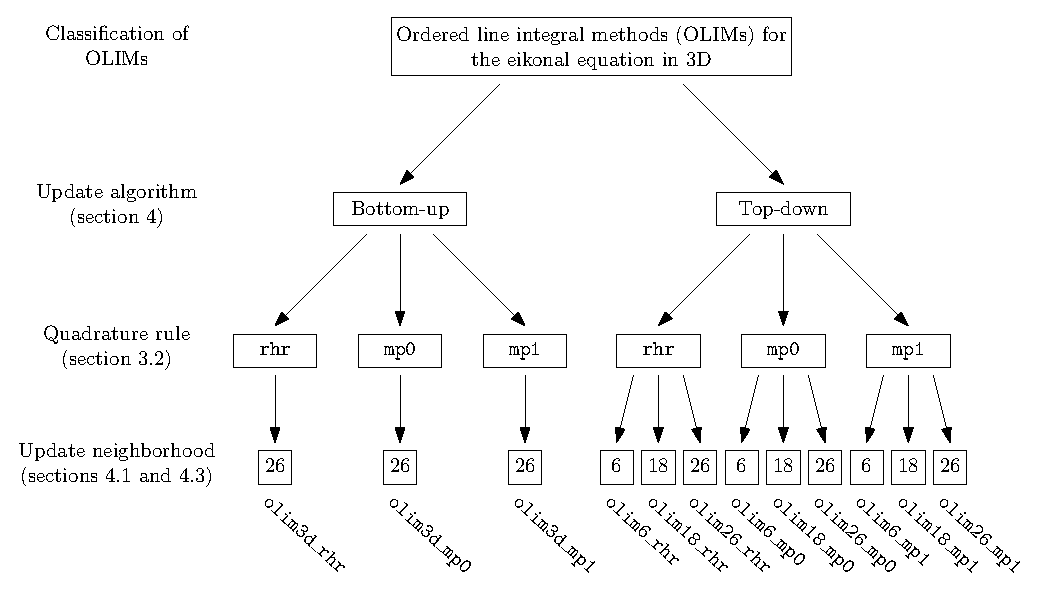
\includegraphics[width=\linewidth]{classification.eps}
  \caption{
    \emph{The family of Dijkstra-like solvers studied in this work.}
    We refer to these as ordered line integral methods (OLIMs).  There
    are three ways of parametrizing the family: by selecting an update
    algorithm, by selecting a quadrature rule, and by (in the case of
    the \emph{top-down} update algorithm, by selecting a neighborhood
    size. Sections in the text that explain these choices in detail
    are indicated. A shorthand notation for referring to each
    parametrized algorithms is listed for each algorithm that is
    involved in numerical tests (e.g., \texttt{olim3d\_mp0}).
  }\label{fig:classification}
\end{figure}

\begin{figure}
  \centering
  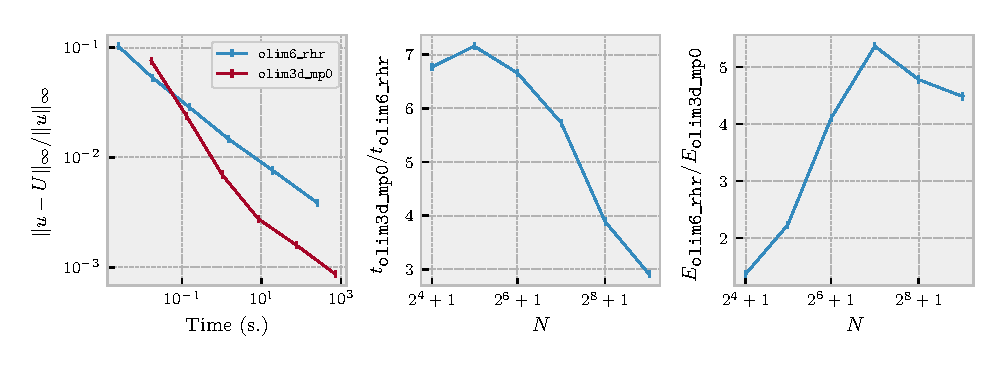
\includegraphics[width=\linewidth]{intro.eps}
  \caption{\emph{Comparing \texttt{olim3d\_mp0} and
      \texttt{olim6\_rhr}.} For the multiple point source problem in
    section\@ \ref{ssec:slotnick} with the domain $\Omega = [0, 1]^3$
    discretized in each direction into $N = 2^p + 1$ (where
    $p = 4, 5, \hdots, 9$); the total number of grid points is
    $N^3$. The plots show from left to right: 1) the relative
    $\ell_\infty$ error plotted vs.\ CPU runtime in seconds, 2)
    quotient of CPU times, 3) quotient of $\ell_\infty$
    errors.}\label{fig:intro}
\end{figure}

Different numerical methods have been proposed for the solution of the
eikonal equation; generally, there are direct solvers and iterative
solvers. The most popular direct solvers are based on Dijkstra's
algorithm (``Dijkstra-like''
solvers)~\cite{tsitsiklis1995efficient,sethian1996fast}, and the most
popular iterative method is the fast sweeping
method~\cite{tsai2003fast,zhao2005fast}. In this work, we develop a
family of Dijkstra-like solvers for the eikonal equation in 2D and 3D,
similar to the fast marching method (FMM) or ordered upwind
methods~\cite{sethian1996fast,sethian2003ordered}. These solvers come
about by discretizing and minimizing the action functional for the
eikonal equation (see section\@ \ref{sec:minimum-action-integral}). The
family of algorithms is parameterized by a choice of update algorithm
(\emph{bottom-up} or \emph{top-down}), quadrature rule (a
righthand rule (\texttt{rhr}), a simplified midpoint rule
(\texttt{mp0}), and a midpoint rule (\texttt{mp1})), and a
neighborhood size (6, 18, or 26 points in 3D). See figure
\ref{fig:classification}. Additionally, we modify our algorithm to
solve the additively factored eikonal equation~\cite{luo2012fast}: to
enhance accuracy, we solve the locally factored eikonal equation near
point sources, which recovers the global $O(h)$ error convergence
expected from a first-order method, where $h > 0$ is the uniform
spacing between grid points. This fixes the degraded
$O(h \log h^{-1})$ convergence often associated with point source
eikonal problems~\cite{qi2018corner} (see~\cite{zhao2005fast} for a
proof of this error bound).

Our \emph{bottom-up} and \emph{top-down} update algorithms
represent two separate approaches to minimizing the number of triangle
and tetrahedron updates that need to be done in 3D, while the
quadrature rules represent a trade-off between speed and accuracy of
the solver. The simplified midpoint rule (\texttt{mp0}) is a sweet
spot that requires extra theoretical justification, which we
provide. Overall, our goal is to explore the relevant algorithm design
trade-offs in 3D and find which solver performs best. Our conclusion
is that, in 3D, \texttt{olim3d\_mp0} is the best overall, and our
results are oriented towards supporting this claim.

Our main results follow:
\begin{itemize}
\item For 3D problems, we develop two separate algorithms: a
  \emph{bottom-up} (\texttt{olim3d}) algorithm, and a \emph{top-down}
  algorithm (\texttt{olim\emph{K}}, where \texttt{\emph{K}}
  \hspace{-0.1em}$=6,18,26$ is the size of neighborhood used). Each
  algorithm locally updates a grid point by performing a minimal
  number of triangle or tetrahedron updates. Depending on the
  quadrature rule, each update is calculated by solving a system of
  nonlinear equations either directly (\texttt{rhr} and \texttt{mp0})
  or iteratively (\texttt{mp1}).
\item We note that this work was done in tandem with research on
  ordered line integral methods for computing the quasipotential 3D
  for nongradient
  SDEs~\cite{dahiya2017ordered,yang2019computing,dahiya2018ordered}. Unlike
  the quasipotential, the eikonal equation is simple enough to allow
  us to analyze and justify our algorithms. We are also able to obtain
  simpler solution methods and established performance guarantees. We
  prove theorems relating our quadrature rules, rigorously justifying
  the \texttt{mp0} rule, establishing it as superior to \texttt{mp1}.
\item We conduct extensive numerical tests on a variety of problems,
  including point source problems for different slowness (index of
  refraction) functions, and multiple point source problems with a
  linear speed function. These problems have analytical solutions,
  which we use as a ground truth.
\item We show that a significant improvement in accuracy is gained
  over the equivalent of the standard fast marching method in 3D
  (\texttt{olim6\_rhr}), and that only modest slowdown is incurred, so
  that our algorithms with improved directional coverage and
  quadrature rules are competitive. See figure \ref{fig:intro} to see
  the improvement of \texttt{olim3d\_mp0} over \texttt{olim6\_rhr},
  and see section\@ \ref{sec:numerical-results} for more details.
\item We use Valgrind~\cite{nethercote2007valgrind} to profile our
  implementation and show that the time spent sorting the heap used to
  order nodes on the front is negligible for all practical problem
  sizes. Since our solvers otherwise run in $O(N^n)$ time, where $n$
  is the dimension of the domain, we suggest that the $O(N^n \log N)$
  cost of the algorithm is pessimistic. Memory access patterns play a
  significant role in scaling.
\end{itemize}

\subsection{Accessing our library} We carefully implement the
algorithms described in this paper using the C++
language~\cite{stroustrup2013c++}. Our library, \texttt{libolim}, can
be accessed from S.\ Potter's website~\cite{sfp-umiacs-homepage}. The
project website includes instructions for downloading and running
basic examples~\cite{libolim-github}. The code used to generate plots
in this paper is also available with
instructions~\cite{libolim-github-plotting}.

\section{Background}\label{sec:background}

\begin{figure}[t]
  \centering
  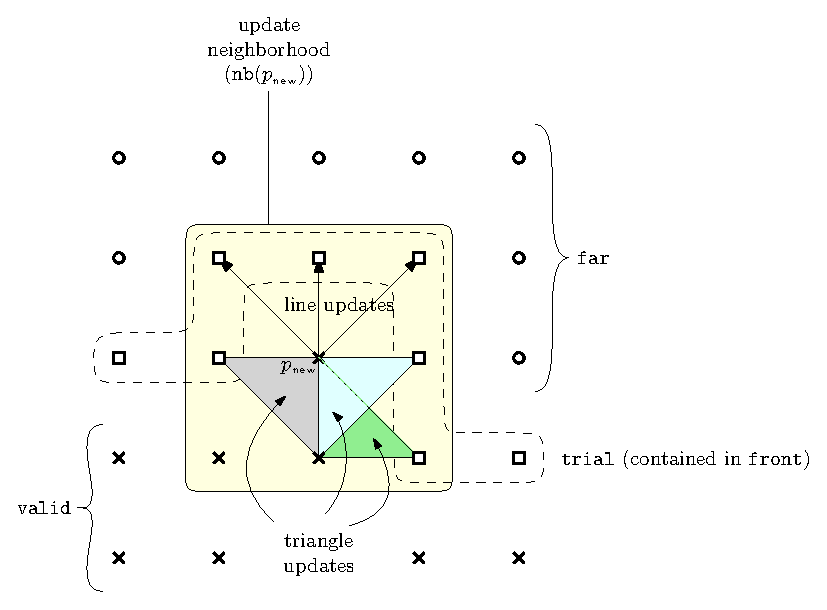
\includegraphics[width=0.9\linewidth]{overview-2.eps}
  \caption{\emph{An overview of a Dijkstra-like algorithm for solving
      the eikonal equation (eq.\@ \ref{eq:eikonal}) in 2D.} See alg.\
    \ref{alg:dijkstra-like} for details. In this diagram, the node
    $\pnew$ has been removed from \texttt{front} and had its state set
    to \texttt{valid}. All \texttt{far} nodes in $\neib(\pnew)$ are
    set to \texttt{trial}, and then all \texttt{trial} nodes in
    $\neib(\pnew)$ are updated. The updates are depicted: there are
    three line updates and three triangles, since it is only necessary
    to perform updates that involve $\pnew$. The OLIM shown here is
    \texttt{olim8}.}
  \label{fig:overview}
\end{figure}

We now provide a brief overview of the eikonal equation and its
numerical solution on a regular grid. We then review the different
algorithms available for its solution, and sketch a generic
Dijkstra-like algorithm which we will refer to throughout the paper to
organize our results. Note that the FMM could be described by this
generic algorithm equally well. Since we focus on Dijkstra-like
algorithms here, our explanation of the fast sweeping and other
iterative methods will be brief.

\subsection{The eikonal equation}

With $n \geq 2$, and given a domain $\Omega \in \R^n$, the eikonal
equation is:
\begin{equation}\label{eq:eikonal}
  \norm{\nabla u(x)} = s(x), \qquad x \in \Omega,
\end{equation}
where $\|\cdot\|$ denotes the $\ell_2$ norm unless otherwise stated,
and $s : \Omega \to (0, \infty)$ is a fixed, positive \emph{slowness
  function}, which forms part of the data. Hence, we solve for
$u : \Omega \to \R_+$. The rest of the boundary data is a subset
$D \subset \Omega$ where $u$ has been fixed; i.e.,
$\left. u \right|_D = g$ for some $g : D \to \R_+$. As an example, if
$s \equiv 1$ and $g \equiv 0$, then the solution of eq.\@ \ref{eq:eikonal} is:
\begin{equation}
  \label{eq:distance-to-Omega}
  u(x) = d(x, D) = \min_{y \in D} \norm{x - y}.
\end{equation}
That is, $u$ is the distance to $D$ at each point in
$\Omega$.

To numerically solve eq.\@ \ref{eq:eikonal}, first let
$\calG = \{p_i\} \subseteq \Omega$ be the set or grid of \emph{nodes}
where we would like to approximate the true solution $u$ with a
numerical solution $U : \calG \to \R_+$. Additionally, for each node
$p \in \calG$, define a set of neighbors,
$\neib(p) \subseteq \calG \backslash \set{p}$. Typically---for the FMM
and \texttt{olim6}, for instance---$\calG$ is taken to be a subset of
a lattice in $\R^n$ and $\neib(p)$ to be each node's $2n$ nearest
neighbors. With $\calG$ defined, we also define the set of
\emph{boundary nodes}, $\boundary \subseteq \calG$. It may happen that
the set $\boundary$ and $D$ do not coincide (e.g., $D$ could be a
curve which does not intersect $\calG$); to reconcile this difference,
the initial value of $U(p)$ for each $p \in \boundary$ must take
$g = \left. u \right|_D$ into account in the best way possible. This
problem has been approached in different ways, and is not the focus of
the present work~\cite{chopp2001some}.

Throughout, we make several simplifying assumptions.
\begin{itemize}
\item All boundary nodes coincide with grid points:
  $\boundary = D \subseteq \calG$.
\item The grid $\calG$ is a regular, uniform grid (a subset of a
  regular, uniform square lattice in 2D or cubic lattice in 3D). We
  denote grid nodes by $x \in \calG$.
\item When numerically computing a new value at a grid point
  $\hat{x} \in \calG$, we transform the neighborhood to the origin and
  scale the vertices so that they have integer values. The transformed
  update node is labeled $\hat{p}$. See section\@ \ref{ssec:quadrature}
  for a detailed explanation.
\end{itemize}

\subsection{Dijkstra-like algorithms}\label{ssec:dijkstra-like}
If we order nodes in $\mathcal{G}$ so that new solution values are
only computed using upwind nodes, the eikonal equation can be solved
directly; i.e., without the use of an iterative solver. This means
that new values of the solution are only involve nodes that have fixed
smaller values. This is done using a variant of Dijkstra's algorithm
for finding shortest paths in a network. Other algorithms which solve
similar network flow problems can also be used, but have different
complexity guarantees~\cite{chacon2012fast}. In particular, Dijkstra's
algorithm is a type of label-setting method for finding shortest paths
in a network; there are also label-correcting
methods~\cite{bertsekas1998network}.

Using Dijkstra's algorithm to solve a ``continuous shortest path''
problem has been discovered in several contexts. The earliest such
development is a theoretical result in computational geometry due to
Mitchell, Mount, and Papadimitriou, who used this idea to compute
exact polyhedral shortest paths (``discrete geodesics'') on
triangulated surfaces~\cite{mitchell1987discrete}. This was followed
by Tsitsiklis who developed a first-order semi-Lagrangian method for
solving isotropic optimal control problems on a uniform
grid~\cite{tsitsiklis1995efficient}. Finally, the fast marching
method, which uses a first-order upwind finite difference scheme was
developed by Sethian for isotropic front
propagation~\cite{sethian1996fast}. Many variations of these methods
have since been
developed~\cite{sethian2003ordered,kao2008legendre}. Our own
development resembles Tsitsisklis's, but extends it past its original
formulation. In particular, Tsitsiklis considers \texttt{olim8\_rhr}
and \texttt{olim26\_rhr}, and does not treat the 3D case in depth. We
generalize this approach, considering higher accuracy quadrature rules
(\texttt{mp0} and \texttt{mp1}) and algorithms which make 3D solvers
fast (our \emph{bottom-up} and \emph{top-down} algorithms).

To write down a generic Dijkstra-like algorithm, there are several
pieces of information which need to be kept track of. A data structure
called \texttt{front} tracks \texttt{trial} nodes while the solver
runs (typically an array-based heap). For each node $p$, apart from
the current value of $U(p)$, the most salient piece of information is
its state, written $p$\texttt{.state}
$\in \set{\texttt{valid}, \texttt{trial}, \texttt{far}}$. To fix
ideas, consider the following high-level Dijkstra-like algorithm:

\begin{algorithm}
  \caption{A generic Dijkstra-like algorithm for solving the eikonal
    equation.}\label{alg:dijkstra-like}
  \begin{enumerate}[nolistsep]
  \item For each $p \in \calG$, set $p$\texttt{.state} $\gets$
    \texttt{far} and $U(p) \gets \infty$.
  \item For each $p \in \boundary$, set $p$\texttt{.state} $\gets$
    \texttt{trial}, and set $U(p)$ to a user-defined value.
  \item While there are \texttt{trial} nodes left in $\calG$:
    \begin{enumerate}[nolistsep]
    \item Let $\pnew$ be the \texttt{trial} node in \texttt{front}
      with the smallest value $U(\pnew)$.\label{enum:get-node}
    \item Set $\pnew$\texttt{.state} $\gets$ \texttt{valid} and remove
      $\pnew$ from \texttt{front}.
    \item For each $\hat{p} \in \neib(\pnew)$, set
      $\hat{p}$\texttt{.state} $\gets$ \texttt{trial} if
      $\hat{p}$\texttt{.state} $=$ \texttt{far}.\label{enum:set-trial}
    \item For each $\hat{p} \in \neib(\pnew)$ such that
      $\hat{p}$\texttt{.state} $=$ \texttt{trial}, update
      $\hat{U} = U(\hat{p})$ and merge $\hat{p}$ into
      \texttt{front}.\label{enum:update-U}
    \end{enumerate}
  \end{enumerate}
\end{algorithm}

Specifying how item \ref{enum:update-U} is to be performed is the crux
of developing a Dijkstra-like algorithm and is left intentionally
vague. This step involves indicating how nodes in $\neib(\hat{p})$ are
used to compute $\hat{U}$, and how they are organized into the
\texttt{front} data structure. The FMM uses an upwind finite
difference scheme where only \texttt{valid} nodes are used to compute
$\hat{U}$, and where nodes on the front are sorted using an
array-based heap implementing a priority
queue~\cite{sethian1996fast}. As an example, Tsitsiklis's algorithm
combines nodes in \texttt{valid} into sets whose convex hulls
approximate the surface of the expanding wavefront and then solves
local raytracing problems where rays emanate from these surfaces. The
method presented here operates in the same way (see figure
\ref{fig:overview}). For specific details, a general reference should
be consulted~\cite{sethian1999level}. In addition to item
\ref{enum:update-U}, algorithm \ref{alg:dijkstra-like} is generic in
the following ways:
\begin{itemize}
\item As we mentioned before, there are different ways of computing
  $\boundary$ and subsequently approximating the initial value of $U$
  for $p \in \boundary$ using
  $g = \left. u \right|_D$~\cite{chopp2001some}
\item How we keep track of the node with the smallest value is
  variable: most frequently, as in Dijkstra's algorithm, a heap
  storing pointers to the nodes is used, leading to $O(N^n \log N)$
  update operations overall, where $N^n$ is the number of nodes. In
  fact, there are $O(N^n)$ variations using Dial's algorithm (a
  bucketed version of Dijkstra's algorithm), but these have not been
  used as extensively as Dijkstra-like
  algorithms~\cite{tsitsiklis1995efficient,kim2001calo,yatziv2006n}.
\item The arrangement of the nodes into a grid or otherwise varies, as
  do the neighborhoods of each node. This affects the update
  procedure. A regular grid is simple to deal with, but Dijkstra-like
  methods have been extended to manifolds and unstructured meshes,
  where the situation is more
  involved~\cite{kimmel1998computing,sethian2000fast,bronstein2008numerical}.
\end{itemize}
Other problems can be solved using Dijkstra-like algorithms: the
static Hamilton-Jacobi equation, an anisotropic generalization of the
eikonal equation, can be solved using the ordered upwind
method~\cite{sethian2003ordered} and other recently introduced
methods~\cite{mirebeau2014efficient,mirebeau2014anisotropic}. Consequently,
the quasipotential of a nongradient stochastic differential equation
can be computed using the ordered line integral method, although the
considerations may be more
involved~\cite{dahiya2017ordered,dahiya2018ordered,yang2019computing}.

\subsection{Fast sweeping methods} Another approach to solving a
discretized version of eq.\@ \ref{eq:eikonal} is the fast sweeping
method~\cite{tsai2003fast,zhao2005fast}. Unlike Dijkstra-like methods,
which are direct solvers, the fast sweeping method is an iterative
solver using an upwind scheme and rotating sweep directions. For
problems where the characteristics of the solution change direction
infrequently, the algorithm obtains $O(N^n)$ complexity. A drawback of
the method is that the constant cannot be bound a priori and depends
heavily on the geometry of the problem. Fast sweeping methods have
been extended to Hamilton-Jacobi
equations~\cite{tsai2003fast,kao2008legendre}, and hybrid methods
combining the fast sweeping method with a Dijkstra-like method have
been introduced recently~\cite{chacon2012fast,chacon2015parallel}.

\section{Ordered line integral methods for the eikonal equation}\label{sec:olim}

The fast marching method~\cite{sethian1996fast} discretizes the
eikonal equation, eq.\@ \ref{eq:eikonal}, and solves this
discretization in an upwind fashion to compute $\hat{U}$. Throughout,
we distinguish between the exact solution $u$ and the numerical
solution $U$, where $\hat{U}$ will always denote the current value to
be computed; likewise, any quantity with a hat (\^{}) will denote a
quantity evaluated at the node being updated. The ordered line
integral method locally and approximately minimizes the minimum action
integral of eq.\@ \ref{eq:eikonal}:
\begin{equation}
  \label{eq:action-functional}
  \hat{u} = \min_{\alpha} \set{u_0 + \int_\alpha s(x) dl},
\end{equation}
where $\alpha$ is a ray parametrized by arc length, $\hat{x}$ is a
target point, $\hat{u} = u(\hat{x})$, and $u_0 = u(\alpha(0))$ (see
section\@ \ref{sec:minimum-action-integral} for a derivation of eq.\
\ref{eq:action-functional}). By constrast, Lagrangian methods (i.e.,
raytracing methods) trace a bundle of rays from a common locus by
integrating Hamilton's equations for the eikonal equation for
different initial conditions. In this section, we describe our
approach to discretizing and approximately minimizing eq.\@
\ref{eq:action-functional}. As we mentioned in section\@
\ref{ssec:dijkstra-like}, to compute $\hat{U} = U(\hat{p})$ in item
\ref{enum:update-U} of algorithm \ref{alg:dijkstra-like}, we need to
approximately minimize several instances of eq.\@
\ref{eq:action-functional}; details of this procedure will be
discussed in section\@ \ref{sec:implementation}. In this section, we
focus on a single instance of the discretized version of eq.\@
\ref{eq:action-functional}, presenting our notation, deriving
prelimary results, and describing the different quadrature rules we
use, detailing useful exact solutions to the approximate minimization
of eq.\@ \ref{eq:action-functional}. We then present theoretical
results.

\begin{figure}
  \centering
  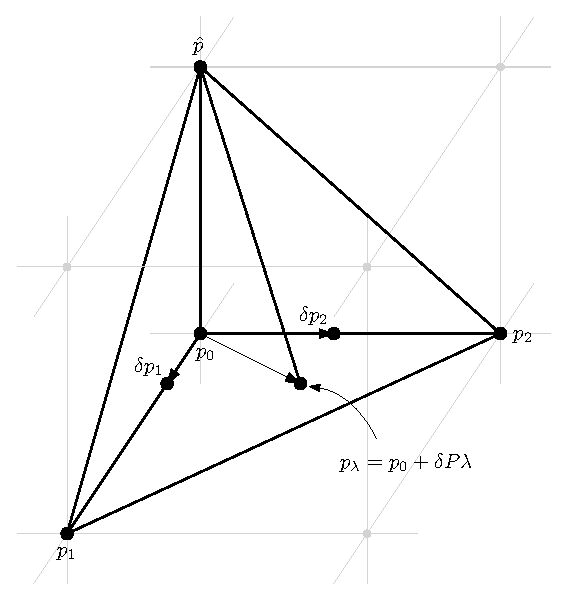
\includegraphics[width=.39864\textwidth]{simplex-diagram-2.eps}
  \hspace{3em}
  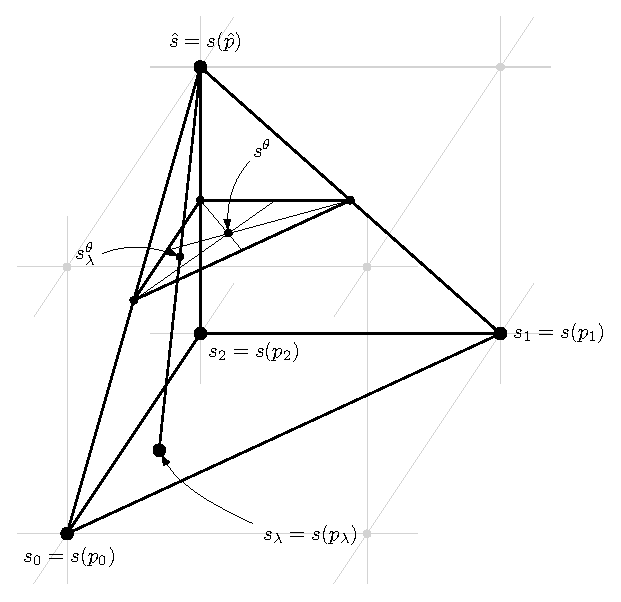
\includegraphics[width=.43912\textwidth]{slowness-tetra-2.eps}
  \caption{\emph{Overview of a tetrahedron update, showing the
      notation in section\@ \ref{sec:olim}}. Left: a point being
    updated, $\hat{p}$, which is identified with the origin, and three
    neighboring points $p_0, p_1$, and $p_2$ that are assumed to be
    \texttt{valid}. The grid $\mathcal{G}$, which contains other
    points in the discretized domain, is highlighted. The domain of
    the minimization problem eq.\@ \ref{eq:constrained-minimization}
    is the convex hull of $p_0, p_1$, and $p_2$. The path minimizing
    eq.\@ \ref{eq:action-functional} is assumed to be the line segment
    connecting $\hat{p}$ and $p_\lambda$. Not pictured is the newly
    \texttt{valid} point $\pnew$, although it is assumed that $\pnew$
    equals one of $p_0, p_1$, or $p_2$. Right: the same update
    tetrahedron, but this time with quantities related to the slowness
    function depicted.}\label{fig:simplex-diagrams}
\end{figure}

\subsection{Approximating the action functional}\label{ssec:quadrature}

In this section we describe how we approximate eq.\@
\ref{eq:action-functional} and reformulate it as a constrained
optimization problem which we solve to update the \texttt{trial} nodes
surrounding a newly \texttt{valid} node $\pnew$.

First, we assume that $\Omega \subseteq \mathbb{R}^n$, where
$n = 2, 3$. The methods presented here work for general $n$. We refer
to each update as a ``simplex update'', since for a dimension $n$, we
need to consider updates of dimensions $d$ where $0 \leq d < n$. For
$n = 3$, we have line updates ($d = 0$), triangle updates ($d = 1$),
and tetrahedron updates ($d = 2$). So, $d$ refers to the dimension of
the base of each simplex, which is the dimension of the domain of the
optimization problem that we will formulate.

We assume that each update simplex is nondegenerate so that a simplex
of dimension $d$ is the convex hull of the update point $\hat{p}$ and
$d$ points $p_0, \hdots, p_{d} \in \neib(\hat{p})$. Since we assume
that our grid $\mathcal{G}$ is uniform and rectilinear, we scale and
translate $\mathcal{G}$ so that $\hat{p} = 0$ and $\|p_i\|_\infty = 1$
for $i = 0, \hdots, d$.

\paragraph{Approximating the integration path with a straight line
  segment.} To approximately minimize eq.\@ \ref{eq:action-functional}
we assume that the minimizing path is a straight line segment
connecting $\hat{p}$ and a point in the convex hull of
$\{p_0, \hdots, p_d\}$, and numerically approximate the action
integral with a quadrature rule. We discuss each part of this
approximation in turn.

We parametrize the ``base of the update simplex'' (the convex hull of
$p_0, \hdots, p_d$), we let $\lambda \in \mathbb{R}^d$ over the set:
\begin{equation}
  \label{eq:lambda}
  \Delta^d = \set{\lambda_i \geq 0 \mbox{ for } i = 1, \hdots, d \mbox{ and } \sum_{i=1}^d \lambda_i \leq 1}.
\end{equation}
If we let $\lambda_0 = \sum_{i=1}^d \lambda_i$, then
$(\lambda_0, \hdots, \lambda_d)$ is a vector of convex coefficients.
Using $\lambda$, we let $\delp_i = p_i - p_0$, define:
\begin{equation}
  \delP = \begin{bmatrix}
    \delp_1 & \cdots & \delp_d
  \end{bmatrix} \in [-1, 1]^{n \times d} \subseteq \mathbb{R}^{n \times d}
\end{equation}
and write a point in the base of the update simplex as:
\begin{equation}
  p_\lambda = p_0 + \sum_{i=1}^d (p_i - p_0) \lambda_i = p_0 + \sum_{i=1}^d \delp_i \lambda_i = p_0 + \delP \lambda.
\end{equation}

We will use the ``$\delta$'' notation for differences and $\lambda$ as
a subscript to denote convex combinations in other contexts, as
well. Throughout, we assume that $U$ is the numerical solution
computed so far at \texttt{valid} points $x \in \mathcal{G}$. Then,
$\delU_i = U_i - U_0 = U(x_i) - U(x_0)$ and
$U_\lambda = U_0 + \delU^\top \lambda$. Likewise,
$\dels_i = s_i - s_0 = s(x_i) - s(x_0)$. By an abuse of notation, we
will think of, e.g., $s_i$, $s(x_i)$, and $s(p_i)$ in the context of
an update as ``the same'', only using the notation $s_i$.

\paragraph{Quadrature rules.} We now turn to approximating the action
integral with different quadrature rules. We consider three different
quadrature rules: a righthand rule (\texttt{rhr}), a simplified
midpoint rule (\texttt{mp0}), and a midpoint rule
(\texttt{mp1}). Recall that we use the hat (\^{}) notation to denote a
quantity that is evaluated at the update point $\hat{p}$:
\begin{align}
  \Frhr(\lambda) &= U_\lambda + \hat{s} h \|p_\lambda\|, \\
  \Fmpzero(\lambda) &= U_\lambda + \parens{\frac{\hat{s} + \tfrac{1}{d+1} \sum_{i=0}^d s_i}{2}} h \|p_\lambda\|, \\
  \Fmpone(\lambda) &= U_\lambda + \parens{\frac{\hat{s} + s_\lambda}{2}} h \|p_\lambda\|.
\end{align}
The difference in the quadrature rules, of course, lies in how we
incorporate the slowness $s$. For $\Frhr$, we evaluate $s$ at the
righthand side of the integral; namely, at $\hat{p}$. For $\Fmpone$,
we evaluate $s$ at the midpoint of the integral, approximating $s$
linearly with the convex combination $s_\lambda$ on the base of the
simplex. Finally, for $\Fmpzero$, we approximate $s_\lambda$ itself
with $s$ evaluated at the centroid of the base of the update simplex,
which is just the arithmetic mean of the $s_i$'s. It will turn out
that $\Fmpzero$ will lead to an inconsistent numerical scheme unless
extra care is taken, which is discussed in the rest of the work.

Note that in the above we use $s_\lambda$ and not $s(p_\lambda)$
because we do not want to assume that we have access to a continuous
functional form for $s$; in most cases, we assume that $s$ will be
provided as gridded data, and that interpolation will be used to
approximate $s$ off-grid.

\paragraph{More general quadrature rules.} The quadrature rules above
are specializations of the following more general quadrature
rules. With $\theta$ such that $0 \leq \theta \leq 1$, we define:
\begin{align}
  F_0(\lambda) &= U_\lambda + \squareb{(1 - \theta)\hat{s} + \frac{\theta}{d+1} \sum_{i=0}^d s_i} h \|p_\lambda\|, \\
  F_1(\lambda) &= U_\lambda + \bigg[ (1 - \theta)\hat{s} + \theta s_\lambda \bigg] h \|p_\lambda\|.
\end{align}
Then, $\Frhr = F_0 = F_1$ with $\theta = 0$, $\Fmpzero = F_0$ with
$\theta = \tfrac{1}{2}$, and $\Fmpone = F_1$ with
$\theta = \tfrac{1}{2}$. We introduce this more general
``$\theta$-rule'' for two reasons:
\begin{itemize}
\item This is a natural geometric generalization, and we wish
  to contextualize our results properly.
\item Our proofs are written in terms of the $\theta$-rules, which
  allows us to provide proofs for $F_0$ and proofs for $F_1$, instead
  of separate proofs for each of $\Frhr$, $\Fmpzero$, and
  $\Fmpone$. As a bonus, our proofs apply to other $\theta$-rules not
  considered here. For instance, schemes using $\theta = 1$ or
  $\theta$ chosen adaptively may be of interest.
\end{itemize}

\subsection{The minimization problem}\label{ssec:minimization-problem}

With $F_0$ and $F_1$ so defined, the minimization problem which
approximates eq.\@ \ref{eq:action-functional-line-segment} to
compute $\hat{U}$ for a fixed update simplex is:
\begin{equation}
  \label{eq:constrained-minimization}
  \hat{U} = \min_{\lambda \in \Delta^d} F(\lambda),
\end{equation}
where $F = \Frhr, \Fmpzero$, or $\Fmpone$. This is a nonlinear,
constrained optimization problem with linear inequality constraints
and no equality constraints (cf.\@ eq.\@ \ref{eq:Delta-LMI}). We
require the gradient and Hessian of $F_0$ and $F_1$ for our algorithms
and analysis. These are easy to compute, but we have found a
particular form for them to be convenient for both implementation and
analysis. The proofs of all propositions and lemmas in this section
can be found in section\@ \ref{sec:minimization-proofs}.

In what follows, we will use the notation:
\begin{equation}
  \proj_p = \frac{p p^\top}{p^\top p}, \qquad \proj_p^\perp = I - \proj_p = I - \frac{p p^\top}{p^\top p}
\end{equation}
for orthogonal projection matrices. Here, $\proj_p$ projects
orthogonally onto $\operatorname{span}(p)$, and $\proj_p^\perp$ onto
its orthogonal complement.

\begin{proposition}\label{prop:F0-grad-and-Hess}
  The gradient and Hessian of $F_0(\lambda; \theta)$ are given by:
  \begin{align}
    \nabla F_0(\lambda) &= \delU + s^{\theta} h \delP^\top \nu_\lambda,\label{eq:F0-grad} \\
    \nabla^2 F_0(\lambda) &= \frac{s^{\theta} h}{l_\lambda} \delP^\top \proj^\perp_{p_\lambda} \delP,
  \end{align}
  where $\nu_\lambda = p_\lambda/l_\lambda$ is the unit vector in the
  direction of $p_\lambda$.
\end{proposition}

\begin{proposition}\label{prop:F1-grad-and-Hess}
  The gradient and Hessian of $F_1(\lambda; \theta)$ satisfy:
  \begin{align}
    \nabla F_1(\lambda) &= \delU + \theta h l_\lambda \dels + s^{\theta}_\lambda h \delP^\top \nu_\lambda, \\
    \nabla^2 F_1(\lambda) &= \set{\delP^\top \nu_\lambda, \theta h \dels} + \frac{s^\theta_\lambda h}{l_\lambda} \delP^\top \proj^\perp_{p_\lambda} \delP, \label{eq:hess-F1}
  \end{align}
  where $\set{a, b} = ab^\top + ba^\top$ is the anticommutator of two
  vectors.
\end{proposition}

Our task is to minimize $F_0$ and $F_1$ over the convex set
$\Delta^n$; so, we need to determine whether $F_0$ and $F_1$ are
convex functions. The next two lemmas address this point.

\begin{lemma}\label{lemma:dPt-cprojp-dP-pd}
  Let $p_0, \hdots, p_d$ form a nondegenerate simplex (i.e.,
  $p_0, \hdots, p_d$ are linearly independent) together with $\hat{p}$
  and assume that $s$ is positive. Then, $\nabla^2 F_0$ is positive
  definite and $F_0$ is strictly convex.
\end{lemma}

For $F_1$, we can only obtain convexity (let alone strict convexity)
for $h$ sufficiently small. For large enough $h$, we will encounter
nonconvex updates. To obtain convexity, we need to stipulate that the
slowness function $s$ be Lipschitz continuous on $\Omega$ with a
Lipschitz constant that is independent of $h$. In practice, we have
not found this to be a particularly stringent restriction.

\begin{lemma}\label{lemma:F-strictly-convex}
  In the setting of lemma \ref{lemma:dPt-cprojp-dP-pd}, additionally
  assume that $s$ is Lipschitz continuous with Lipschitz constant
  $K \leq C$ on $\Omega$, for some constant $C > 0$ independent of
  $h$. Then, $\nabla^2 F_1$ is positive definite (hence, $F_1$ is
  strictly convex) for $h$ small enough.
\end{lemma}

We have found that all \texttt{mp1} updates become strictly convex
problems rapidly as $h \to 0$. The reason for this is discussed at the
end of section\@ \ref{ssec:causality}.

\subsection{Validation of \texttt{mp0}}\label{ssec:validation}

If we consider an update simplex defined by the nodes
$p_0, \hdots, p_{n-1}$, each subset of these nodes defines another,
lower-dimensional update simplex, which lies on the boundary of the
original simplex. For example, three triangle updates form the
boundary of a single tetrahedron update. We expect the values of $F_i$
to be the same on the surface of the neighborhood without regard to
the simplex under consideration (note that the update simplexes share
common lower-dimensional boundaries). Likewise, we expect $F_i$ to be
continuous as we transfer between adjacent simplexes. For $F_1$ this
is the case, but for $F_0$ with $\theta \neq 0$, the function $F_0$
may not be well-defined or continuous at boundaries. This problem can
lead to inconsistent and divergent solvers. A heuristic fix is to
first minimize eq.\@ \ref{eq:constrained-minimization} for $F_0$
with nonzero $\theta$ to obtain the minimizing argument $\lambda^*_0$,
then set $\hat{U} = F_1(\lambda_0^*)$; i.e., to replace $F_0$ with
$F_1$ for the purposes of evaluation, or to use $F_0$ as a surrogate
when minimizing $F_1$.

If we use Newton's method to minimize $F_1$, starting from
$\lambda_0^*$ and letting $\lambda_1^*$ denote the optimum of eq.\@
\ref{eq:constrained-minimization} for $F_1$, then we can use the
convergence theory of Newton's method to bound the distance between
$\lambda_0^*$ and $\lambda_1^*$, thereby bounding the error incurred
by using \texttt{mp0} instead of \texttt{mp1}.

\begin{theorem}\label{thm:mp0-newton}
  Using lemma \ref{lemma:F-strictly-convex}, let $h$ be sufficiently
  small so that $F_1$ is strictly convex. Then, the error
  $\dellam^* = \lambda_1^* - \lambda_0^*$ satisfies
  $\norm{\dellam^*} = O(h)$. Further, if we let
  $\lambda_0 = \lambda_0^*$ in the following Newton iteration:
  \begin{equation}
    \label{eq:lam0-iter-to-lam1}
    \lambda_{k+1} \gets \lambda_k - \nabla^2 F_1(\lambda_k)^{-1} \nabla F_1(\lambda_k), \qquad k = 0, 1, \hdots,
  \end{equation}
  then this iteration is well-defined, and converges quadratically to
  $\lambda_1^*$. This immediately implies that the error incurred by
  \texttt{mp0} is $O(h^3)$ per update compared to \texttt{mp1}; i.e.:
  \begin{equation}
    \label{eq:mp0-error}
    \abs{F_1(\lambda_1^*) - F_1(\lambda_0^*)} = O(h^3).
  \end{equation}
\end{theorem}

\begin{proof}
  The proof of theorem \ref{thm:mp0-newton} is detailed in appendix
  \ref{app:validation-proofs}.
\end{proof}

We can provide some intuition for why this bound is satisfactory. If
we assume that our domain is spanned along a diameter by $O(N)$ nodes,
and that $h \sim N^{-1}$, then we can anticipate $O(N)$ downwind
updates, starting from $\boundary$ and extending to the boundary of
$\calG$ in any direction. Accumulating the error over these nodes, we
can expect the maximum pointwise error between a solution to eq.\@
\ref{eq:eikonal} computed by using \texttt{mp0} and \texttt{mp1} to be
$O(h^2)$, which is dominated by the $O(h)$ discretization error coming
from the linear convergence of the method itself. Hence, using
\texttt{mp0} instead of \texttt{mp1} to find the parameter $\lambda$
(i.e., determine the local characteristic) should introduce no
significant error when evaluating $F_1$.

% If we exchange the roles of $F_0$ and $F_1$ (if we start from
% $\lambda_1^*$ and perform a Newton iteration on $\nabla F_0$) we can
% obtain the foregoing error bound again. The main reason to start from
% $\lambda_0^*$ and iterate to $\lambda_1^*$ is that it allows us to use
% \texttt{mp0} to initialize \texttt{mp1}. Indeed, in the next section,
% we will see that it is possible to perform \texttt{mp0} updates
% without resorting to a nonlinear solver, but that this is not the case
% for \texttt{mp1}. For $d = 0$, this is unimportant, but for
% $d \geq 1$, minimizing $F_0$ can be cheaper. Reducing the number of
% $F_1$ update iterations leads to a sped-up method with the same
% accuracy.

\subsection{Exact solution for \texttt{rhr} and \texttt{mp0}}\label{ssec:exact-soln}

Since $F_0$ is strictly convex, $\nabla F_0(\lambda) = 0$ is
sufficient for the optimality of $\lambda$, if we ignore the
constraint $\lambda \in \Delta^d$. The unconstrained system of
nonlinear equations defined by $\nabla F_0(\lambda) = 0$ can be solved
exactly without an iterative solver. We can compute the solution using
the reduced QR decomposition of $\delP$ and by considering the
problem's geometry (see figure \ref{fig:f0-exact}). This is captured
in the following theorem. We will discuss how to use this theorem
efficiently in a solver in section\@
\ref{ssec:algorithms-and-skipping}.

\begin{theorem}\label{thm:f0-exact}
  Let $\delP = QR$ be the reduced QR decomposition of $\delP$; i.e.,
  where
  $Q \in \mathbb{R}^{n \times d}, R \in \mathbb{R}^{d \times d},
  Q^\top Q = I_d$, and with $R$ upper triangular. For $s^\theta, h$,
  and $U$ fixed, if
  $\lambda^* = \argmin_{\lambda \in \mathbb{R}^n}
  F_0^\theta(\lambda)$, then:
  \begin{align}
    l_{\lambda^*} &= \sqrt{\frac{p_0^\top {(I - QQ^\top)} p_0}{1 - \norm{R^{-\top} \frac{\delU}{s^\theta h}}^2}},\label{eq:l-star-expression} \\
    \lambda^* &= -R^{-1} \parens{Q^\top p_0 + l_{\lambda^*} R^{-\top} \frac{\delU}{s^\theta h}},\label{eq:f0-exact-lambda} \\
    \hat{U} &= U_0 + \frac{s^\theta h}{l_{\lambda^*}} p_0^\top p_{\lambda^*}.\label{eq:f0-exact}
  \end{align}
\end{theorem}

\begin{proof}
  See section\@ \ref{sec:exact-soln-proofs}.
\end{proof}

\subsection{Equivalence of the upwind finite difference scheme and
  $F_0$}\label{ssec:equivalence}

If we linearly approximate $U$ near $\hat{p}$, then for
$i = 0, \hdots, n - 1$, we find that $\hat{U}$ approximately
satisfies:
\begin{equation}
  \label{eq:finite-differences}
  U_i - \hat{U} = \nabla \hat{U}^\top p_i.
\end{equation}
This finite difference approximation to eq.\@ \ref{eq:eikonal} can
be solved exactly and is a known generalization of the upwind finite
difference scheme used by the fast marching method to an unstructured
mesh~\cite{kimmel1998computing,sethian2000fast}. Computing $\hat{U}$
using this approximation is equivalent to solving:
\begin{equation}
  \hat{U} = \min_{\lambda \in \Delta^n} F_0(\lambda)
\end{equation}
in a sense made precise by the following theorem.

\begin{theorem}[Equivalence of upwind finite difference scheme and $F_0$]\label{thm:equivalence}
  Let $\hat{U}$ by the solution of eq.\@
  \ref{eq:finite-differences} and let
  $\hat{U}' = \min_{\lambda \in \R^n} F_0(\lambda)$. Then, $\hat{U}$
  exists if and only if $\|R^{-\top} \delU\| \leq s^\theta h$, and can
  be computed from:
  \begin{equation}
    \label{eq:U-finite-diff}
    \hat{U} = U_i - p_i^\top Q R^{-\top} \delU + \norm{\pmin} \sqrt{{(s^\theta h)}^2 - \norm{R^{-\top} \delU}^2},
  \end{equation}
  where $\pmin = (I - QQ^\top) p_i$ (for all
  $i = 0, \hdots, n - 1$---see figure \ref{fig:f0-exact} in section\@
  \ref{sec:exact-soln-proofs}). Additionally, the following hold:
  \begin{enumerate}
  \item The finite difference solution and line integral solution
    coincide: i.e., $\hat{U} = \hat{U}'$ can be computed from:
    \begin{equation}
      \label{eq:U-from-Ui-exact}
      \hat{U} = U_i + s^\theta h p_i^\top \nu_{\lambda^*},
    \end{equation}
    where $\lambda^* = \argmin_{\lambda \in \R^n} F_0(\lambda)$ and
    $\nu_{\lambda^*} = p_{\lambda^*}/l_{\lambda^*}$.
  \item The characteristics found by solving the finite difference
    problem and minimizing $F_i$ coincide and are given by
    $[p_{\lambda^*}, \hat{p}] = [p_{\lambda^*}, 0]$.
  \item The approximated characteristic passes through
    $\conv(\set{p_0, \hdots, p_{n-1}})$ if and only if
    $\lambda^* \in \Delta^n$.
  \end{enumerate}
\end{theorem}

\begin{proof}
  See section\@ \ref{sec:equivalence-proofs}.
\end{proof}

\subsection{Causality}\label{ssec:causality} Dijkstra-like
methods are based on the idea of monotone causality, similar to
Dijkstra's method itself. To compute shortest paths in a network,
Dijkstra's method uses dynamic programming to compute globally optimal
shortest paths using local information~\cite{dijkstra1959note}. In
this way, the distance to each downwind vertex must be greater than
its upwind neighboring vertices. To ensure convergence to the correct
viscosity solution, our scheme must be consistent and
monotone~\cite{crandall1983viscosity}. Our OLIMs using the
\texttt{rhr} quadrature rule inherit the consistency and causality of
the finite difference methods which they are equivalent to if they use
the same 4 (in 2D) or 6 (in 3D) point neighborhoods. Since we consider
many different update neighborhoods involving distinct simplexes, we
provide a simple way of checking whether each simplex is causal.

The causality of an update depends on the underlying simplex and the
problem data. In particular, an update is causal for $F_i$ if:
\begin{equation}
  \hat{U} = F_i(\lambda_i^*) \geq \max_i U_i.
\end{equation}
It is enough to determine whether or not each type of update simplex
admits only causal updates, which relates to whether the simplex is
acute.

We also consider something we refer to here as the ``update gap'': the
difference $\hat{U} - \max_i U_i$. As discussed in Tsitsiklis's
original paper~\cite{tsitsiklis1995efficient}, an alternative to
Dijkstra's algorithm is Dial's algorithm---a bucketed version of
Dijkstra's algorithm which runs in $O(N^n)$ time, where the constant
depends on the bucket size~\cite{dial1969algorithm,kim2001calo}. In
this case, the size of the buckets is determined by the update gap. It
is unclear whether there is any real advantage of a Dial-like solver
(see~\cite{jeong2008fast} for a discussion); indeed, we present
numerical evidence suggesting that this is not the case in section\@
\ref{ssec:impl-notes}. Despite this, the update gap is of fundamental
importance and limits the number of nodes that can be processed in
parallel without violating causality.

\begin{theorem}\label{thm:causality}
  For $\nu_i = p_i/\|p_i\|$, an update simplex is causal for $F_0$ if
  and only if $\nu_i^\top \nu_j \geq 0$ for all $i$ and $j$ such that
  $0 \leq i < n$ and $0 \leq j < n$. If we assume that $s$ is
  Lipschitz continuous, for $h$ small enough, the simplex is also
  causal for $F_1$, and the term in $F_1$ which prevents an update
  from being causal decays with order $O(h^2)$. Furthermore, the
  update gap is given explicitly by:
  \begin{equation}
    \hat{U} - \max_i U_i = s^\theta h \min_{i, j} \frac{\nu_i^\top \nu_j}{\norm{p_i}}.
  \end{equation}
\end{theorem}

\begin{proof}
  See section\@ \ref{sec:causality-proofs}.
\end{proof}

\noindent The fact that our methods are causal for all practical
problem sizes follows from the fact that the term preventing causality
decays rapidly---see eq.\@ \ref{eq:F1-in-terms-of-F0}. This can be
seen easily by rewriting $F_1(\lambda)$ as $F_0(\lambda)$ plus a small
perturbation (which is $O(h^2)$) and using the Lipschitz continuity of
$s$.

\subsection{Local factoring}

Near rarefaction fans, for example if $D$ is a point source or the
domain contains obstacles with corners, the rate of convergence of the
eikonal equation is diminished. For the eikonal equation with point
source data and constant slowness, this degrades the rate of
convergence to $O(h \log
h^{-1})$~\cite{qi2018corner,zhao2005fast}. Different factored eikonal
equations which treat this problem have been
developed~\cite{fomel2009fast,luo2012fast}. In this section, we show
how the ordered line integral method can be easily adapted to additive
factoring, and provide numerical tests that show that it recovers the
expected linear rate of convergence for factored problems. Our focus
is locally factored point sources, but this approach can be applied to
the globally factored equation and other types of rarefaction fans
occuring at corners or discontinuities~\cite{qi2018corner}.

\begin{figure}
  \centering
  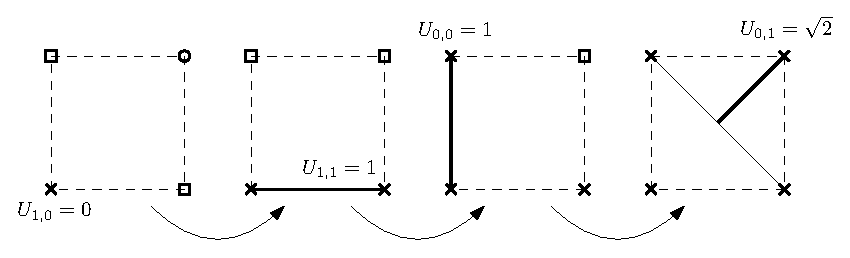
\includegraphics[width=\linewidth]{factoring-example.eps}
  \caption{\emph{An example of running \texttt{olim4\_rhr} with local
      factoring for three steps.} Note that \texttt{olim4\_rhr} is
    equivalent to the standard FMM in 2D. Ordered clockwise from the
    top left, the nodes are $p_{0, 0}, p_{0, 1}, p_{1, 1}$, and
    $p_{1, 0}$, with $h = 1$ (so we assume our domain is identified
    with $\mathbb{Z}^2$). We assume a constant slowness function:
    $s \equiv 1$. Initially, $p^\circ = p_{1, 0}$ is the only node in
    \texttt{bd} and is factored. The first two steps proceed exactly
    the same as for the unfactored method, since the steps between the
    source nodes and the updated nodes lie along characteristics of
    the solution, $u$. In the third step, the unfactored method would
    set $U_{0,1} \gets 1 + \nicefrac{\sqrt{2}}{2}$. For the factored
    method, since $\tau_{0,1} = 1 - 1 = 0 = \tau_{1,0}$, we find that
    $U_{0,1} \gets 0 + s^\circ l^\circ_{\nicefrac{1}{2}} + s^\theta h
    l_{\nicefrac{1}{2}} = \nicefrac{\sqrt{2}}{2} +
    \nicefrac{\sqrt{2}}{2} = \sqrt{2}$.}\label{fig:factoring-example}
\end{figure}

Let $x^\circ \in \Omega$ be the location of a point source so that
$\boundary = \set{x^\circ}$ and let the grid
$\calG \subseteq \mathbb{Z}^n$ be aligned so that
$p^\circ \in \mathbb{Z}^n$; that is, we let $p^\circ$ be the image of
$x^\circ$ in the update neighborhood, in the same way that each $p_i$
is the image of a grid point $x \in \calG$ (hence, $p^\circ$ varies
from update to update, but $x^\circ$ remains the same). For a point
$p_\lambda$, define $l^\circ_\lambda = \norm{p_\lambda - p^\circ}$ and
let $s^\circ = s(x^\circ)$. The additive factorization of $U$ around
$x^\circ$ is~\cite{luo2012fast,qi2018corner}:
\begin{align}
  U(x) = T(x) + \tau(x), \qquad \text{where} \qquad T(x) = s^\circ \norm{x - x^\circ},
\end{align}
i.e.\ $u_\lambda = T_\lambda + \tau_\lambda$ where
$T_\lambda = s^\circ h l^\circ_\lambda$. Our original definition of
$F_i^\theta$ was such that $\hat{U} = F_i^\theta(\lambda^*)$. We will
define $G_i^\theta$ analogously. Letting
$\tau_\lambda = \tau_0 + \deltau^\top \lambda$, where $\tau_i$ and
$T_i$ are the values of $\tau$ and $T$ at $p_i$ for each $i$, we
define:
\begin{align}
  \label{eq:Gi}
  G_0(\lambda) = G_0^\theta(\lambda) &= \tau_\lambda + T_\lambda + s^\theta h l_\lambda, \\
  G_1(\lambda) = G_1^\theta(\lambda) &= \tau_\lambda + T_\lambda + s^\theta_\lambda h l_\lambda.
\end{align}
Like with $F_0$ and $F_1$, the only difference between
$G_0$ and $G_1$ is between the terms containing
$s^\theta$ and $s^\theta_\lambda$.

To solve the factored eikonal equation, we choose a factoring radius
$\rfac$, replacing $F_i$ with $G_i$ in eq.\@
\ref{eq:constrained-minimization} for nodes which lie within a
distance $\rfac$ of $x^\circ$. For constant slowness, the effect of
this is to solve eq.\@ \ref{eq:eikonal} exactly inside of the
locally factored region. For clarity, this is depicted in figure
\ref{fig:factoring-example}. Algorithm \ref{alg:top-down} can be
applied to solve eq.\@ \ref{eq:constrained-minimization} for
factored nodes. The gradient and Hessian of $G_i$ are simple
modifications of the gradient and Hessian for $F_i$.

\begin{lemma}
  The gradient and Hessian of $G_i$ for $i = 0, 1$ are given
  by:
  \begin{align}
    \label{eq:G-grad-hess}
    \nabla G_i(\lambda) &= \nabla F_i(\lambda) - \deltau + \frac{s^\circ h}{l^\circ_\lambda} \delP^\top {(p_\lambda - p^\circ)}, \\
    \nabla^2 G_i(\lambda) &= \nabla^2 F_i(\lambda) + \frac{s^\circ h}{l^\circ_\lambda} \delP^\top \proj^\perp_{p_\lambda - p^\circ} \delP.
  \end{align}
\end{lemma}

\section{Implementation of the ordered line integral
  method}\label{sec:implementation}

\begin{figure}
  \centering
  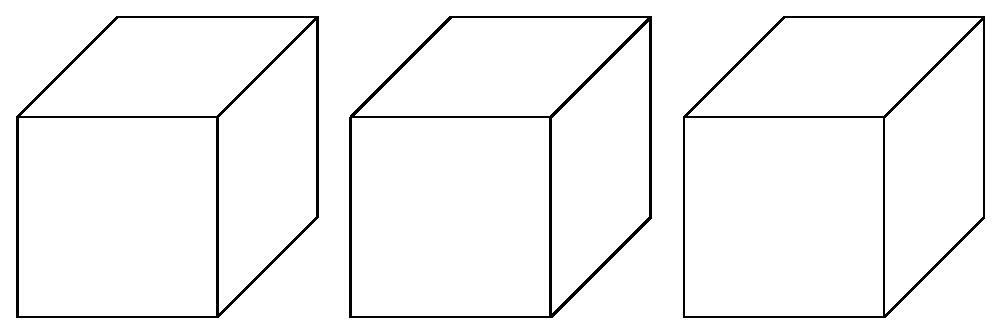
\includegraphics[width=0.95\linewidth]{neighborhoods.eps}
  \caption{\emph{Neighborhoods for the \emph{top-down} family of algorithms.}
    Algorithms \texttt{olim4} and \texttt{olim8} are 2D solvers and
    the rest are 3D solvers. The color coding of tetrahedron updates
    is the same for this figure and figure \ref{fig:octant-numbering}
    below.}\label{fig:neighborhoods}%
  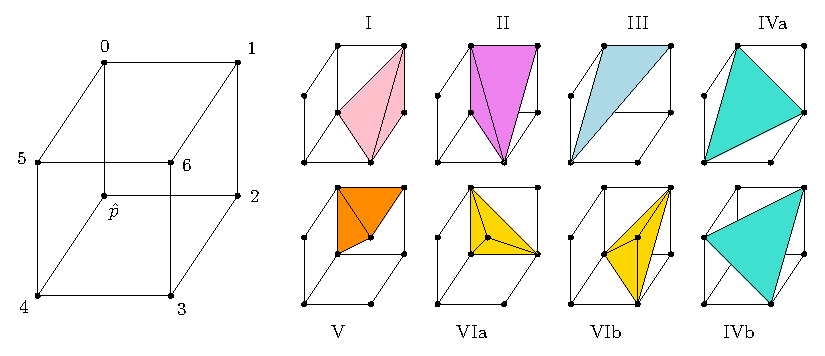
\includegraphics[width=0.95\linewidth]{simplex-groups.eps}
  \caption{\emph{Numbering scheme for update groups for the \emph{top-down} solvers.} In this
    diagram, $\hat{p}$ is being updated. The diagonally opposite node
    is the sixth (last) node, with the other six nodes numbered 0--5
    cyclically.}\label{fig:octant-numbering}
  { \footnotesize
    \vspace{1em}
    \begin{tabular}{c|cccccc|cccccc|cccccc|cc}
      0 & $\groupmarker$ & & & & $\groupmarker$ & $\groupmarker$ & $\groupmarker$ & & & $\groupmarker$ & & $\groupmarker$ & $\groupmarker$ & & $\groupmarker$ & & & $\groupmarker$ & $\groupmarker$ & \\
      1 & $\groupmarker$ & $\groupmarker$ & & & & $\groupmarker$ & $\groupmarker$ & $\groupmarker$ & & & $\groupmarker$ & & $\groupmarker$ & $\groupmarker$ & & $\groupmarker$ & & & & $\groupmarker$ \\
      2 & $\groupmarker$ & $\groupmarker$ & $\groupmarker$ & & & & & $\groupmarker$ & $\groupmarker$ & & & $\groupmarker$ & & $\groupmarker$ & $\groupmarker$ & & $\groupmarker$ & & $\groupmarker$ & \\
      3 & & $\groupmarker$ & $\groupmarker$ & $\groupmarker$ & & & $\groupmarker$ & & $\groupmarker$ & $\groupmarker$ & & & & & $\groupmarker$ & $\groupmarker$ & & $\groupmarker$ & & $\groupmarker$ \\
      4 & & & $\groupmarker$ & $\groupmarker$ & $\groupmarker$ & & & $\groupmarker$ & & $\groupmarker$ & $\groupmarker$ & & $\groupmarker$ & & & $\groupmarker$ & $\groupmarker$ & & $\groupmarker$ & \\
      5 & & & & $\groupmarker$ & $\groupmarker$ & $\groupmarker$ & & & $\groupmarker$ & & $\groupmarker$ & $\groupmarker$ & & $\groupmarker$ & & & $\groupmarker$ & $\groupmarker$ & & $\groupmarker$ \\
      \multicolumn{1}{c}{} & \multicolumn{6}{c}{I} & \multicolumn{6}{c}{II} & \multicolumn{6}{c}{III} & \multicolumn{2}{c}{IV}
    \end{tabular} \\
    \vspace{1em}
    \begin{tabular}{c|cccccc|cccccc|ccc}
      0 & $\groupmarker$ & & & & & $\groupmarker$ & $\groupmarker$ & & & & $\groupmarker$ & & $\groupmarker$ & & \\
      1 & $\groupmarker$ & $\groupmarker$ & & & & & & $\groupmarker$ & & & & $\groupmarker$ & & $\groupmarker$ & \\
      2 & & $\groupmarker$ & $\groupmarker$ & & & & $\groupmarker$ & & $\groupmarker$ & & & & & & $\groupmarker$ \\
      3 & & & $\groupmarker$ & $\groupmarker$ & & & & $\groupmarker$ & & $\groupmarker$ & & & $\groupmarker$ & & \\
      4 & & & & $\groupmarker$ & $\groupmarker$ & & & & $\groupmarker$ & & $\groupmarker$ & & & $\groupmarker$ & \\
      5 & & & & & $\groupmarker$ & $\groupmarker$ & & & & $\groupmarker$ & & $\groupmarker$ & & & $\groupmarker$ \\
      6 & $\groupmarker$ & $\groupmarker$ & $\groupmarker$ & $\groupmarker$ & $\groupmarker$ & $\groupmarker$ & $\groupmarker$ & $\groupmarker$ & $\groupmarker$ & $\groupmarker$ & $\groupmarker$ & $\groupmarker$ & $\groupmarker$ & $\groupmarker$ & $\groupmarker$ \\
      \multicolumn{1}{c}{} & \multicolumn{6}{c}{V} & \multicolumn{6}{c}{VI} & \multicolumn{3}{c}{VII}
    \end{tabular}%
  }
  \caption{\emph{Tables of update groups.} These tables should be
    scanned columnwise: each column of dots selects a different
    tetrahedron. Tetrahedra (0, 1, 2), (2, 3, 4), and (4, 5, 0) in
    group I and all tetrahedra in group VII are degenerate and can be
    omitted.}\label{fig:tetrahedra-groups}
\end{figure}

In this section, we describe our \emph{bottom-up} and \emph{top-down}
algorithms. We emphasize the 3D solver, since in 2D, the distinction
between the two is less important. Each algorithm reduces the number
of updates that are done without degrading solution accuracy by using
an efficient enumeration or search of the neighboring simplexes. The
difference between the algorithms is in how this is done.

In section\@ \ref{ssec:simplex-enumeration}, we start by showing how
to enumerate update tetrahedra and put them into separate groups of
congruent tetrahedra. By only performing updates from these groups, we
obtain \emph{top-down} algorithms with stencils of different sizes. Our
numerical tests (section\@ \ref{sec:numerical-results}) will show how
neighborhoods of different sizes lead to different patterns of
directional coverage, which can significantly affect the error. We
also discuss the update gaps attainable using these tetrahedron groups
in section\@ \ref{ssec:update-gaps}.

Following this, we describe our \emph{bottom-up} algorithm in section\@
\ref{ssec:bottom-up-search}, which involves first finding the minimal
update of smallest dimension ($d = 0$, a line update), then finding
the minimal update of the next highest dimension ($d = 1$, a triangle
update) which is incident to the original update, and so on. In 3D,
this means finding the minimal line update, doing neighboring triangle
updates which contain the minimal line update, and then neighboring
tetrahedron updates which contain the minimal triangle update. We can
think of this algorithm as a fast search for the first arrival
characteristic.

To minimize the number of updates that are done, it is important to
take advantage of the structure of the underlying constrained
optimization problems that are being solved in order to skip
unnecessary lower or higher dimensional updates. We describe this
procedure in section\@ \ref{ssec:algorithms-and-skipping}. How this
is done varies depending on the choice of quadrature rule
(\texttt{mp0}, \texttt{mp1}, or \texttt{rhr}) and type of algorithm
(\emph{bottom-up} or \emph{top-down}).

\subsection{Simplex enumeration for the \emph{top-down}
  algorithm}\label{ssec:simplex-enumeration}

When a node is first removed from \texttt{front} and has just become
\texttt{valid} (item \ref{enum:get-node}), an isotropic solver must do
updates involving, at the very least, the node's $2n$ von Neumann
neighbors. We can use larger neighborhoods to improve the accuracy of
the result. Doing so does not necessarily improve the order of
convergence of the solver, but can significantly improve the accuracy
of the solution. For all of the solvers considered in this paper, in
3D, we only ever consider neighborhoods with at most 26 neighbors.

For the \emph{top-down} solver, we simplify things by treating a node's
neighboring octants separately. That is, we iterate over each octant
and do all updates that lie inside that octant before moving onto the
next. To do this, we enumerate all update tetrahedra with vertices
$p \in \{0, 1\}^3$ in a symmetric fashion. Since we assume our update
tetrahedra have been translated so that $\hat{p} = 0 \in \mathbb{Z}^n$
(see section\@ \ref{ssec:quadrature}), this means enumerating
${7 \choose 3} = 35$ choices of vertices. Some choices lead to
degenerate tetrahedra (i.e., such that $p_0, p_1$, and $p_2$ are
linearly dependent), so the number of nondegenerate update tetrahedra
is fewer than 35 per octant. This makes it reasonable to write out the
update procedure as straight-line code.

We enumerate the tetrahedra in a type of ``shift-order'' (see, e.g.,
\cite{arndt2010matters})---that is, we start with an unseen bit
pattern, and group this pattern together with all of its shifts (with
rotation). This groups the tetrahedra into sets that are rotationally
symmetric about the diagonal of the octant. In our implementation, we
conditionally compile different groups so that no unnecessary
branching is done. This is done using C++
templates~\cite{stroustrup2013c++}. Example stencils for the versions
of \texttt{olim6}, \texttt{olim18}, and \texttt{olim26} that are used
for our numerical test are shown in figure
\ref{fig:neighborhoods}. The tetrahedron groups are shown in figures
\ref{fig:octant-numbering} and \ref{fig:tetrahedra-groups}.

\subsection{Update gaps for tetrahedron
  groups}\label{ssec:update-gaps}

If we apply theorem \ref{thm:causality} to the tetrahedron groups
enumerated in figures \ref{fig:octant-numbering} and
\ref{fig:tetrahedra-groups}, we get the following update gaps
(ignoring the $s^\theta h$ factor): \vspace{0.5em}
\begin{center}
  \begin{tabular}{lc|lc|lc|lc}
    Group I & $\nicefrac{1}{\sqrt{2}}$ & Group II & $\nicefrac{1}{\sqrt{2}}$ & Group III & $\nicefrac{1}{\sqrt{2}}$ & Group IVa & 0 \\
    \midrule
    Group V & $\nicefrac{1}{\sqrt{3}}$ & Group VIa & 0 & Group VIb & $\boldsymbol{\nicefrac{2}{\sqrt{3}}}$ & Group IVb & $\nicefrac{1}{\sqrt{2}}$
  \end{tabular}
\end{center}
\vspace{0.5em} The idea of the update gap is first explored in
Tsitsiklis's original paper~\cite{tsitsiklis1995efficient}; in this
work, the fact that Group IVa has no update gap and that the update
gap of Group V is $1/\sqrt{3}$ is noted and an $O(N^n)$ algorithm
based on Dial's algorithm is presented using Group V for the update
tetrahedra. This same observation is made in a more recent paper
explicitly detailing a method based on Dial's
algorithm~\cite{kim2001calo}. A method based on a combination of
tetrahedra groups will have as its update gap the minima of each of
the individual groups' update gaps. We note here that a solver based
on a combination of Groups I and VIb has a larger update gap than a
solver based on Group V. This should have a positive impact on the
performance of any parallel Dijkstra-like method.

\subsection{The search procedure used by the \emph{bottom-up}
  algorithm}\label{ssec:bottom-up-search}

Another approach is to take advantage of the fact that lower
dimensional updates provide some information about the likely
direction of arrival of the first arrival time characteristic. If we
know where the minimum line update is, then the characteristic is
nearby. Starting with the minimum line update, we enumerate
neighboring vertices and perform the corresponding triangle updates,
then enumerate vertices which are sufficiently close to the minimum
triangle update, doing any relevant tetrahedron updates along the way.

\begin{figure}[t]
  \centering
  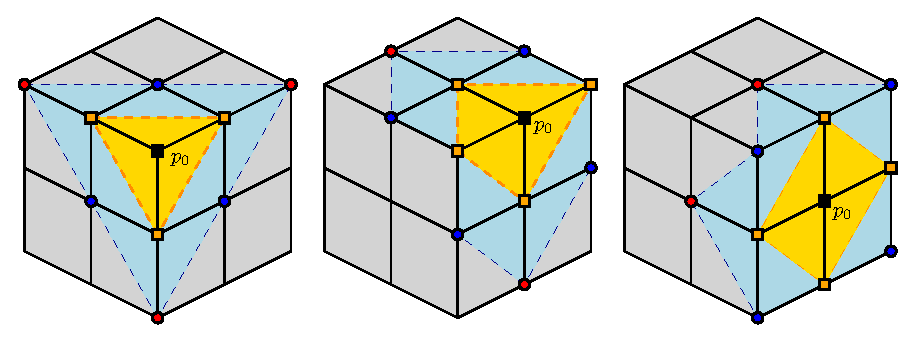
\includegraphics[width=0.85\linewidth]{hu-neighborhoods.eps}
  \caption{\emph{The three types of neighborhoods for the \emph{bottom-up}
      algorithm with $q_1 = 1 = q_2$, $d_1 = 1$, and $d_2 = 2$.} The
    yellow and blue regions indicate where triangle and tetrahedron
    updates may be performed, respectively. For instance, with $p_0$
    the minimizing line update vertex, candiates for $p_1$ consist of
    the yellow nodes: triangle updates involving these candidates and
    $p_0$ will be performed. Once a yellow node ($p_1$) has been
    selected, tetrahedron updates involving the neighboring blue nodes
    (candidates for $p_2$) will be performed. Note that the updates
    performed correspond roughly to a combination of groups I, V, VIa,
    and VIb.}\label{fig:hu-neighborhoods}
\end{figure}


\begin{figure}
  \centering
  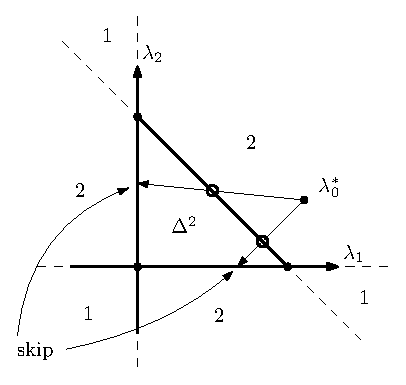
\includegraphics[width=0.4\linewidth]{skip-zones.eps}
  \caption{\emph{Skipping lower-dimensional updates when solving the
      unconstrained minimization problem.} For $d = 2$, if
    $\lambda_0^* \in \Delta^2$, all three triangle updates can be
    skipped. On the other hand, when minimizing $F_0$ using theorem
    \ref{thm:f0-exact}, if $\lambda^*_0 \notin \Delta^2$ and depending
    on where $\lambda_0^*$ lies, it is possible to skip one or two
    triangle updates. In this case, we label the different regions by
    the number of updates that it is possible to skip: $\lambda^*$
    here lies in a region labeled ``2'', since it is possible to skip
    the two triangle updates on the opposite side of $\Delta^2$. Along
    the same lines, if $\lambda^*$ were to lie in a region labeled
    ``1'', two triangle updates would be ``visible'', and it would
    only be possible to skip one update.}\label{fig:skip-zones}
\end{figure}

While the \emph{top-down} algorithm is parametrized by the choice of
tetrahedron groups to include, the \emph{bottom-up} algorithm is parametrized
by the norms used to search for neighboring vertices as well as the
permitted search radii. In 3D, let $p_0$ be the vertex that admits the
minimum line update; then, $p_1$ must satisfy
$\norm{p_1 - p_0}_{q_1} \leq d_1$, where $q_1 = 1, 2$, or $\infty$ and
$d_1$ is a positive integer. Likewise, when searching for tetrahedron
updates, for a candidate vertex $p_2$, we require
$\norm{p_2 - p_1}_{q_2} \leq d_2$ and
$\norm{p_2 - p_0}_{q_2} \leq d_2$ to hold simultaneously.

For our numerical tests, we use the $\ell_1$ norm in both cases
($q_1 = 1 = q_2$), and set $(d_1, d_2) = (1, 2)$ (see figure
\ref{fig:hu-neighborhoods}). We found this choice of parameters to be
a good compromise between speed and accuracy. Using larger
neighborhoods does lead to a more accurate solution, but causes the
solver to run more slowly. We do not explore the effect of this
parametrization in this paper, since our choice of parameters performs
well enough already (see section\@ \ref{sec:numerical-results}).
\subsection{Minimization algorithms and skipping
  updates}\label{ssec:algorithms-and-skipping}

Performing an update is the same as solving eq.\@
\ref{eq:constrained-minimization} for fixed problem data. When
$F_i = F_0$, we can use theorem \ref{thm:f0-exact} or
\ref{thm:equivalence} to compute $\lambda_0^*$. In this case,
$\lambda_0^*$ may lie outside $\Delta^d$. On the other hand, if
$F_i = F_1$, we need to use an algorithm that can solve the
constrained optimization problem defined by eq.\@
\ref{eq:constrained-minimization}. Our approach has been to use
sequential quadratic programming (SQP), although there are many other
options~\cite{bertsekas1999nonlinear,nocedal2006numerical}. It is
possible to skip some updates; and, indeed, the performance of our
algorithms depends on this happening. We skip updates in three
different ways. The first two strategies for skipping updates are used
by the \emph{top-down} algorithms, and the third is used by the \emph{bottom-up}
family of algorithms.

\paragraph{\emph{top-down} constrained skipping} When computing an update
using a constrained solver, we can rule out all incident
lower-dimensional updates, since we have computed the global
constrained optimum on $\Delta^d$.

\paragraph{\emph{top-down} unconstrained skipping} If we do an update using
an unconstrained solver, then depending on where the optimum
$\lambda_0^*$ lies, we can skip some lower-dimensional updates. The
idea is simple: since $F_0$ is strictly convex, if we consider a
straight line starting at $\lambda_0^*$ and extending in some
direction, then $f$ restricted to that line is monotonically
increasing as we move away from $\lambda_0^*$. Hence, for a
tetrahedron update, if $\lambda_0^* \notin \Delta^2$, then we can skip
all updates which are not ``visible'' (in parameter space) from
$\lambda_0^*$. This is illustrated in the figure \ref{fig:skip-zones}.

\paragraph{\emph{Bottom-up} KKT skipping} We can also skip higher-dimensional
updates. For example, if we do the three triangle updates on the
boundary of a tetrahedron update, we can use the Karush-Kuhn-Tucker
necessary conditions for optimality of a constrained optimization
problem~\cite{nocedal2006numerical} to determine if the minimizer on
the boundary is also a global minimizer for the constrained
minimization problem given by eq.\@
\ref{eq:constrained-minimization}. Let
$L(\lambda, \mu) = F_i(\lambda) + (A\lambda - b)^\top \mu$ be the
Lagrangian function, where $\mu \in \mathbb{R}^{d + 1}$ is the vector
of Lagrange multipliers. Since $F_0$ is strictly convex and since we
assume $h$ is small enough for $F_1$ to be strictly convex, if
$\lambda^*$ lies on the boundary of $\Delta^d$, we only need to check
that the optimum Lagrange multipliers $\mu^*$ are dual feasible; i.e.,
whether
$\mu^* \geq 0$~\cite{bertsekas1999nonlinear,nocedal2006numerical}. For
$\lambda^* \in \partial \Delta^d$, letting
$\mathcal{I} = \set{i : (A\lambda - b)_i = 0}$ be the set of active
constraints' indices, stationarity requires:
\begin{equation}\label{eq:stationarity}
  A^\top_{\mathcal{I}} \mu_{\mathcal{I}}^* = \nabla F_i(\lambda).
\end{equation}
See eq.\@ \ref{eq:Delta-LMI} for the definition of $A$; the
notation $A_{\mathcal{I}}$ refers to the submatrix consisting of rows
of $A$ indexed by $\mathcal{I}$. For a tetrahedron update in 3D,
$A \in \mathbb{R}^{3 \times 2}$ and $|\mathcal{I}| \leq 2$ (not all
three constraints be active simultaneously). In particular, if
$i \notin \mathcal{I}$, then $\mu_i^* = 0$, and otherwise, $\mu_i^*$
can be computed easily from eq.\@ \ref{eq:stationarity}. Once the
full vector of Lagrange multipliers has been computed, if
$\mu^* \geq 0$, then the update may be skipped. A modified version of
this strategy for skipping updates was used in our work on computing
the quasipotential for nongradient SDEs in
3D~\cite{yang2019computing}.

\subsection{The \emph{bottom-up} and \emph{top-down} algorithms}\label{ssec:top-down-and-bottom-up}

\begin{algorithm}[t]
  \caption{The \emph{top-down} algorithm.}\label{alg:top-down}
  \textbf{Input:} the neighboring update points $(p_0, \hdots, p_d)$,
  and, for $i = 0, \hdots, d$, the downwind solution value
  $U_i = U(p_i)$ and the slowness $s_i = s(p_i)$. \\
  \textbf{Output:} a new solution value $\hat{U} = U(\hat{p})$, where
  $\hat{U} > U_i$ for $i = 0, \hdots, d$.
  \begin{enumerate}[nolistsep]
  \item Set $\hat{U} \gets \infty$.
  \item Initialize $\calV_d$ according to eq.\@ \ref{eq:calU} for
    each $d = 0, \hdots, n - 1$.
  \item For $d = n - 1$ down to $0$:
    \begin{enumerate}
    \item For each $(p_0, \hdots, p_d) \in \calV_d$:
      \begin{enumerate}
      \item If $F_i = F_0$ (\texttt{mp0} or \texttt{rhr}):
        \begin{enumerate}
        \item Compute $U$ for $(p_0, \hdots, p_{d})$ using theorem
          \ref{thm:f0-exact} or \ref{thm:equivalence}.
        \item Remove updates from $\calV_0, \hdots, \calV_{d-1}$ by
          visibility (see figure \ref{fig:skip-zones}).
        \end{enumerate}
      \item Otherwise, if $F_i = F_1$ (\texttt{mp1}):
        \begin{enumerate}
        \item Compute $U$ by solving eq.\@
          \ref{eq:constrained-minimization} numerically (we use SQP).
        \item Remove all lower-dimensional updates from
          $\calV_0, \hdots, \calV_{d-1}$.
        \end{enumerate}
      \item Set $\hat{U} \gets \min(\hat{U}, U)$.
      \end{enumerate}
    \end{enumerate}
  \end{enumerate}
\end{algorithm}

\begin{algorithm}[t]
  \caption{The \emph{bottom-up} algorithm.}\label{alg:bottom-up}
  \textbf{Input:} for $i = 0, \hdots, d$, the update point $p_i$, the
  values
  $U_i = U(p_i)$, and $s_i = s(p_i)$. \\
  \textbf{Output:} the new solution value $\hat{U} = U(\hat{p})$.
  \begin{enumerate}[nolistsep]
  \item Set $\hat{U} \gets \infty$ and $p_0 \gets \pnew$.
  \item For $i = 1, \hdots, n - 1$:
    \begin{enumerate}
    \item For each \texttt{valid} $p_i$ close enough to
      $p_0, \hdots, p_{i-1}$ (see section\@
      \ref{ssec:bottom-up-search}), do the update corresponding to
      $(p_0, \hdots, p_i)$ and keep track of the minimizing
      $\lambda^* \in \Delta^i$. This update can optionally be skipped
      by first computing $\mu^*$ corresponding to the optimum of the
      incident lower-dimensional update $(p_0, \hdots, p_{i-1})$ and
      checking if $\mu^* \geq 0$.\label{enum:bottom-up-for}
    \item Let $p_i$ be the node which forms the update with the
      minimum value.
    \item If $F_i = F_0$ (\texttt{mp0} or \texttt{rhr}), compute $U$
      for $(p_0, \hdots, p_{i})$ using theorem \ref{thm:f0-exact} or
      \ref{thm:equivalence}.
    \item Otherwise, if $F_i = F_1$ (\texttt{mp1}), compute $U$ for
      $(p_0, \hdots, p_{i})$ by solving eq.\@
      \ref{eq:constrained-minimization}.
    \item Set $\hat{U} \gets \min(\hat{U}, U)$.
    \end{enumerate}
  \end{enumerate}
\end{algorithm}

In this section, we describe our \emph{bottom-up} and \emph{top-down} algorithms. We
note for clarity that these algorithms correspond to item
\ref{enum:update-U} of algorithm \ref{alg:dijkstra-like}.

To describe our \emph{top-down} algorithm (see algorithm \ref{alg:top-down}),
we define:
\begin{equation}\label{eq:calU}
  \begin{aligned}
    \calV_d = \big\{\set{p_0, \hdots, p_d}: \; &p_i\texttt{.state}=\texttt{valid} \mbox{ for } i = 0, \hdots, d, \\
    &\mbox{and } \set{p_0, \hdots, p_d} \mbox{ belongs to the selected update group}, \\
    &\mbox{and } \pnew \in \set{p_0, \hdots, p_d} \big\}
  \end{aligned}
\end{equation}
for $d = 0, \hdots, n - 1$. These sets collect all possible simplex
updates: i.e., updates which both belong to a group as defined in
section\@ \ref{ssec:simplex-enumeration} and are \texttt{valid}. The
third condition is an important optimization. To see why it is
correct, fix an update set $\calV_d$. If $\set{p_0, \hdots, p_d}$
satisfies the first two conditions but not the third, we can see that
$\hat{p}$ would have already been updated from it in a previous
iteration. All new information affecting $\hat{U}$ during this
iteration must be computed from an update involving $\pnew$.

The \emph{bottom-up} algorithm (algorithm \ref{alg:bottom-up}) builds up each
update $(p_0, \hdots, p_d)$ one vector at a time by searching for
adjacent minimizing updates of higher dimension. The optimization
involving $\pnew$ described above can be incorporated by initially
setting $p_0 \gets \pnew$.

\section{Numerical Results}\label{sec:numerical-results} We test on several different
slowness functions with available exact solutions for point source
data, and a linear speed function (i.e., $1/s$) which has been shown
to be amenable to local factoring. For each quadrature rule described
in section\@ \ref{ssec:quadrature} (\texttt{mp0}, \texttt{mp1}, or
\texttt{rhr}), we have two 2D algorithms, \texttt{olim4} and
\texttt{olim8}, corresponding to 4-\ and 8-point stencils,
respectively. Since there is no advantage in 2D, we don't apply the
\emph{top-down} or \emph{bottom-up} approaches. In 3D, we have three \emph{top-down}
algorithms: \texttt{olim6} (group IVa), \texttt{olim18} (groups I,
IVa, and IVb), and \texttt{olim26} (group V). We also test the
\emph{bottom-up} algorithm \texttt{olim3d} (see figure
\ref{fig:hu-neighborhoods}).

\subsection{Implementation Notes}\label{ssec:impl-notes}

\begin{figure}
  \centering 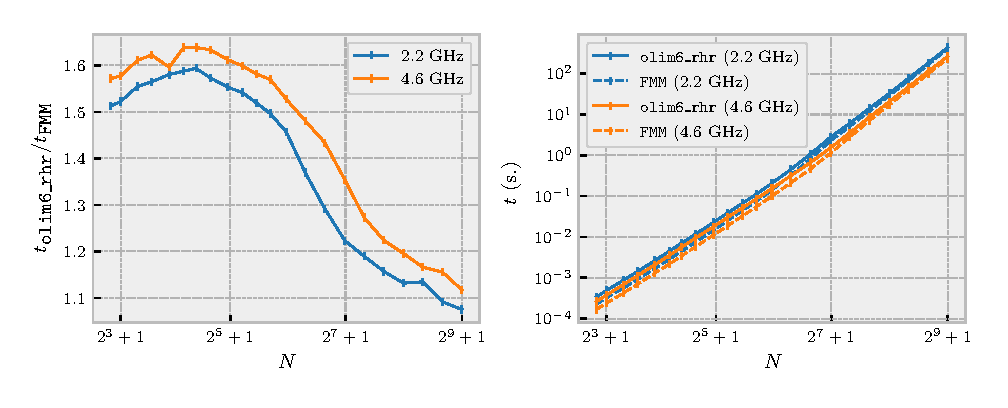
\includegraphics[width=\linewidth]{speed-comparison.eps}%
  \caption{\emph{Slowdown incurred by using \texttt{olim6\_rhr}
      instead of the FMM.} From left to right: 1) the ratio of
    runtimes versus $N$, 2) the total CPU runtime of each solver. We
    compare results on two different computers: ``2.2 GHz'' is a 2015
    MacBook Air with a 2.2 GHz Intel Core i7 CPU, 8 GB of 1600 MHz
    DDR3 RAM, a 256 KiB L2 cache, and a 4 MiB L3 cache; ``4.6 GHz'' is
    a custom built workstation running Linux with a 4.6 GHz Intel Core
    i7 CPU, 64 GB of 2133 MHz DDR4 RAM, a 1536 KiB L2 cache, and 12
    MiB L3 cache. Both computers have 32 KiB L1 instruction caches and
    data caches. The plots here use our standard $\Omega = [-1, 1]^3$
    domain discretized into $N = 2^p + 1$ nodes in each direction,
    with $s \equiv 1$ and a point source at the
    origin.}\label{fig:speed-comparison}
\end{figure}

\begin{figure}
  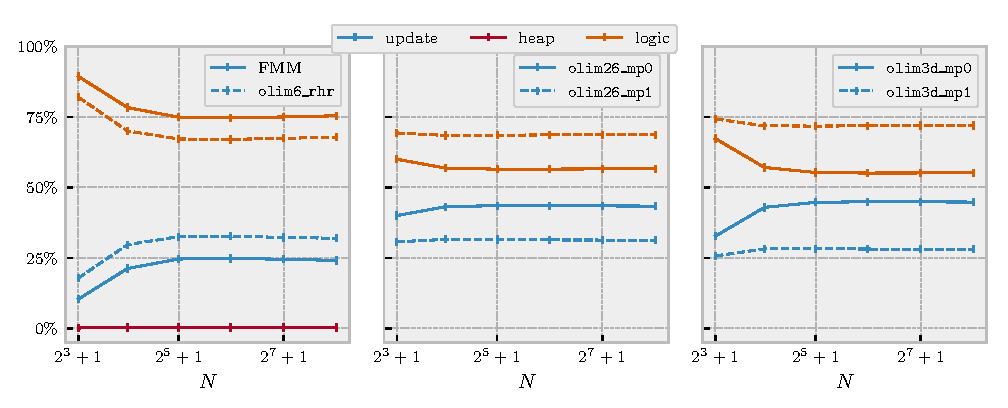
\includegraphics[width=\linewidth]{tasks.eps}%
  \caption{\emph{Percentage of time spent on different tasks as
      determined by profiling.} The ``update'' tasks and ``heap''
    tasks are clearly defined, while the ``logic'' task contains a
    variety of things related to control-flow, finding neighbors, and
    memory movement---basically, the parts of algorithm
    \ref{alg:dijkstra-like} that don't clearly pertain to computing
    new $\hat{U}$ values or keeping \texttt{front} updated. From these
    plots, it is clear that memory speed plays a large role in
    determining efficiency. To some extent, even though the more
    complicated update procedures are slower, their slowness is hidden
    somewhat by memory latency as problem sizes grow. For large $N$
    and some solvers (the middle and right plots), ``heap'' takes too
    little time, and is not picked up by the
    profiler.}\label{fig:tasks}
\end{figure}

Before describing our numerical tests, we briefly comment on our
implementation and make some observations about its performance. A
discussion of some of the choices that we made in our implementation
follows:
\begin{itemize}
\item We precompute and cache all values of $s$ on the grid $\calG$,
  as opposed to reevaluating $s$, because we assume that $s$ will be
  provided as gridded data (consider, e.g., the shape from shading
  problem~\cite{kimmel2001optimal}, where the input data is an image).
\item We maintain \texttt{front} using a priority queue implemented
  using an array-based heap, which is updated using the \texttt{sink}
  and \texttt{swim} functions described in Sedgewick and
  Wayne~\cite{sedgewick2011algorithms}.
\item We store \texttt{front} as a dense grid of states: for each node
  in $p \in \calG$, we track $p$\texttt{.state} for all time for every
  node. We could implement a sparse \texttt{front} using a hash map or
  a quadtree or octree, which would save space, but would also be much
  slower to update. In fact, since updating these data structures
  frequently takes $O(\log n)$ time, using a sparse front has the
  potential to degrade the overall complexity to $O(n \log^2 n)$.
\end{itemize}

We use a policy-based design~\cite{alexandrescu2001modern} written in
the C++ programmed language which makes heavy use of templates. This
allows us to conditionally compile different features and reuse logic
to implement different Dijkstra-like algorithms. In particular, we
implement the standard FMM~\cite{sethian1996fast} and make a direct
comparison between it and the ordered line integral method which it is
equivalent to, \texttt{olim6rhr} (see figure
\ref{fig:speed-comparison}). We have found that only a modest slowdown
is incurred by using \texttt{olim6rhr} for problems of moderate
size. The disparity between the two is greater for smaller problem
sizes, which is due to cache effects.

Using Valgrind~\cite{nethercote2007valgrind}, we profiled running our
solver on the numerical tests below for different problem sizes and
categorized the resulting profile data. See figure
\ref{fig:tasks}. The ``update'' task corresponds to time spent
actually computing updates, the ``logic'' task is a grab bag category
for time spent on program logic, and ``heap'' corresponds to updating
the array-based heap which implements \texttt{front}. Since the
asymptotic complexity of the ``update'' and ``logic'' sections is
$O(N^n)$, and since ``heap'' is $O(N^n \log N)$, we can see from
figure \ref{fig:tasks} that since so little time is spent updating the
heap, \emph{the algorithm's runtime is better thought of as $O(N^n)$
  for practical problem sizes.} This is a consequence of using an
array-based heap, which is cheap to update, and a dense grid of
states, which can be read from and written to in $O(1)$ time.

\subsection[Single point source]{Slowness functions with an analytic
  solution for a point source}\label{ssec:point-source-problems}

\begin{figure}
  \centering 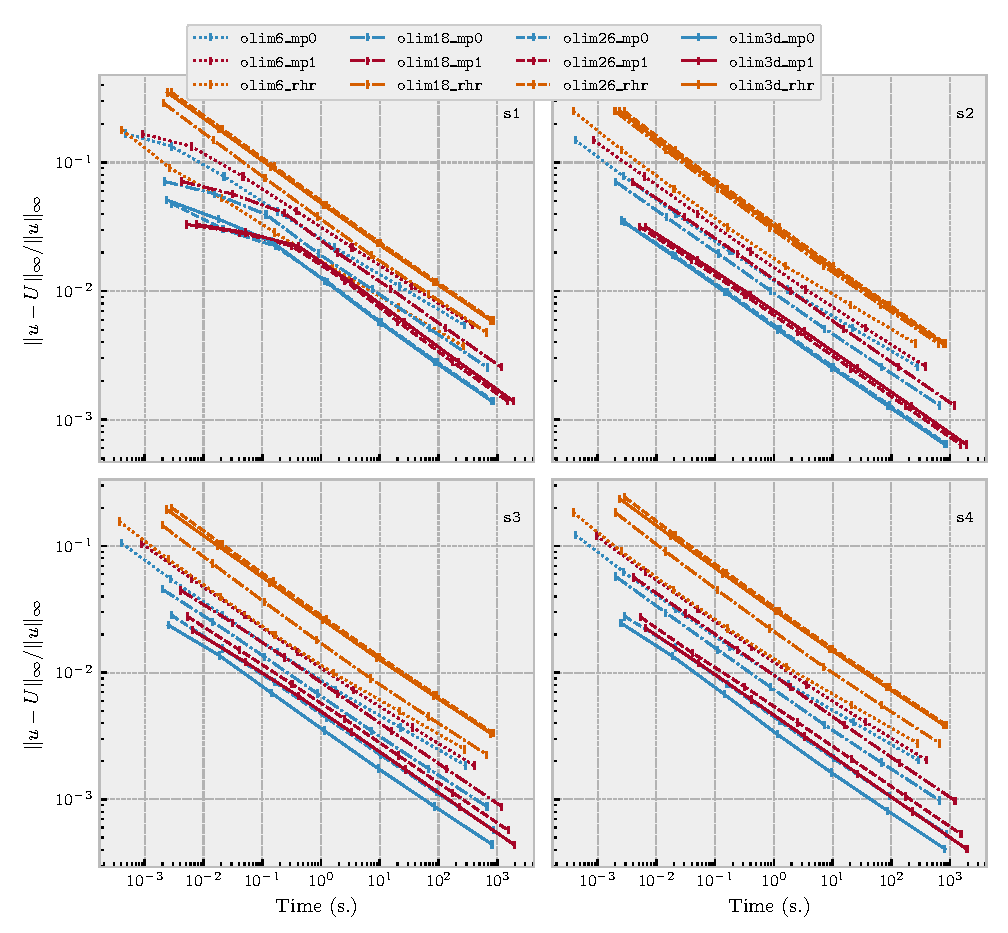
\includegraphics[width=\linewidth]{time_vs_error_3d.eps}
  \caption{\emph{Relative $\ell_\infty$ error plotted against CPU
      runtime in seconds.} The domain is $\Omega = [-1, 1]^3$
    discretized uniformly in each direction into $N = 2^p + 1$ points,
    where $p = 3, \hdots, 9$, so that there are $N^3$ points
    overall. The slowness functions used are listed in section\@
    \ref{ssec:point-source-problems}. We note that the horizontal and
    vertical axes of each subplot are the
    same.}\label{fig:time-vs-error}
\end{figure}

\begin{figure}
  \centering 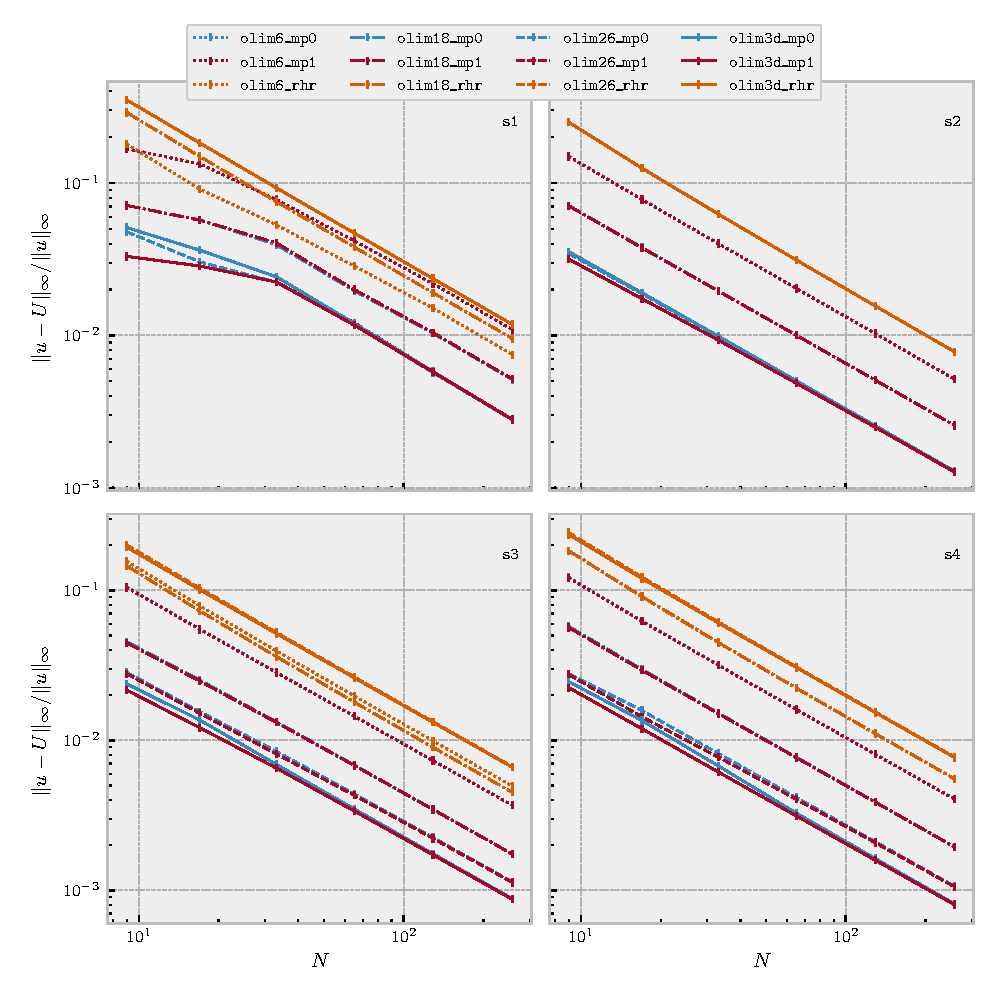
\includegraphics[width=\linewidth]{size_vs_error_3d.eps}
  \caption{\emph{Relative $\ell_\infty$ error plotted versus $N$.} The
    setup is the same as in figure \ref{fig:time-vs-error}, except
    that $p = 3, \hdots, 8$, so that the largest $N$ is $257$ instead
    of $513$. For \texttt{olim26} and \texttt{olim3d}, we can see that
    \texttt{mp0} is initially less accurate than \texttt{mp1} but
    quickly attains parity, in accordance with theorem
    \ref{thm:mp0-newton}. For \texttt{olim6} and \texttt{olim18}, the
    error is the same between \texttt{mp0} and \texttt{mp1} for all
    slowness functions, so these plots
    overlap.}\label{fig:size-vs-error}
\end{figure}

Using eq.\@ \ref{eq:eikonal} directly, a simple recipe to create
pairs of slowness functions and solutions is to prescribe a continuous
function $u$ with level sets homeomorphic to balls and compute
$s(x) = \norm{\nabla u(x)}_2$ analytically, which is valid for a
single point source at the origin. Such tests allow us to observe the
effect of local factoring, and to see how \texttt{mp0}, \texttt{mp1},
and \texttt{rhr} compare. The following table lists our test
functions: \vspace{0.5em}
\begin{center}
  \begin{tabular}{cccc}
    Name & $u(x)$ & $s(x)$ \\
    \midrule
    \texttt{s1} & $\cos(r) + r - 1$ & $1 - \sin(r)$ \\
    \texttt{s2} & $r^2/2$ & $r$ \\
    \texttt{s3} & $S(x)^\top A S(x)$ & $\alpha\norm{\operatorname{diag}(C(x)){(A + A^\top)}S(x)}$ \\
    \texttt{s4} & $\tfrac{1}{2} x^\top A^{1/2} x$ & $\norm{x}_A = \sqrt{x^\top A x}$
  \end{tabular}
\end{center}
\vspace{0.5em} We assume that $x \in \Omega = [-1, 1]^3$. We also
define $r = \norm{x}$, and vector fields
$S(x) = (\sin(\alpha x_i))_{i=1}^3$ and
$C(x) = (\cos(\alpha x_i))_{i=1}^3$; we take $\alpha = \pi/5$. For
\texttt{s3} and \texttt{s4}, we assume that $A$ is symmetric positive
definite. In 3D, the matrices we use for \texttt{s3} and \texttt{s4}
are:\begin{equation} A_{\texttt{s3}} = \begin{bmatrix}
    1 & \nicefrac{1}{4} & \nicefrac{1}{8} \\
    \nicefrac{1}{4} & 1 & \nicefrac{1}{4} \\
    \nicefrac{1}{8} & \nicefrac{1}{4} & 1
  \end{bmatrix} = A_{\texttt{s4}}^{1/2}
\end{equation}

Our results are displayed in figures \ref{fig:time-vs-error} and
\ref{fig:size-vs-error}. We include plots of relative $\ell_\infty$
error plotted versus problem size and time, as well as $\ell_\infty$
error plotted versus $N$. We summarize our observations:
\begin{itemize}
\item For \texttt{rhr}, as we increase directional coverage
  (\texttt{olim6\_rhr} $\to$ \texttt{olim18\_rhr} $\to$
  \texttt{olim26\_rhr}), the error constant does not improve; in fact,
  for \texttt{s1}, \texttt{s3}, and \texttt{s4}, increasing the
  directional coverages causes the accuracy to deteriorate (see figure
  \ref{fig:size-vs-error}). This can be due to the fact that the
  errors due to quadrature and due to linear interpolation have
  different signs, and may partially compensate each other (e.g., in
  \texttt{olim6}), and that this balance may worsen with increased
  directional coverage, leading to a reduction in interpolation error.
  On the other hand, using one of the midpoint rules allows improved
  directional coverage to translate into an improved error constant.
\item If we scan each graph horizontally, we can see that the
  difference in error between \texttt{mp0} and \texttt{mp1} is
  minimal. For each \texttt{mp1} graph, the corresponding \texttt{mp0}
  graph has the same error, but is shifted to the left, reflecting the
  fact that the \texttt{mp0} OLIMs are substantially faster. This is
  consistent with theorem \ref{thm:mp0-newton}, which justifies the
  use of \texttt{mp0}.
\item With respect to the choice of neighborhood, \texttt{olim6} is
  the fastest; and, for each choice of neighborhood, \texttt{mp0}
  provides the best combination of speed and accuracy. If we are
  willing to pay somewhat in speed, we can dramatically improve the
  error constant by improving the directional coverage and using a
  solver like \texttt{olim3d\_mp0}. This tradeoff is more pronounced
  for smaller problem sizes. A theme running through this work is
  that, as the problem size increases, memory access patterns come to
  dominate the runtime, and the disparity between the faster and
  slower neighborhoods becomes less pronounced. To see this, compare
  the start of each graph in the top-left of the plots, and their ends
  in the bottom-right. We can observe, e.g., that the maximum
  horizontal distance between starting points and ending points has
  decreased significantly, which confirms this observation.
\item Our high accuracy algorithms allow us to obtain a better
  solution on rough grids: this is helpful since opportunities to
  refine the mesh are limited in 3D. Discretizing $\Omega = [-1, 1]^2$
  in each direction into $N = 2^{14} + 1$ nodes requires about as much
  memory as discretizing $\Omega = [-1, 1]^3$ with $N = 2^{9} + 1$,
  which leads to $h$ being 32 times smaller in 2D than in 3D.
\end{itemize}

\subsection{A linear speed function}\label{ssec:slotnick}

\begin{figure}
  \centering
  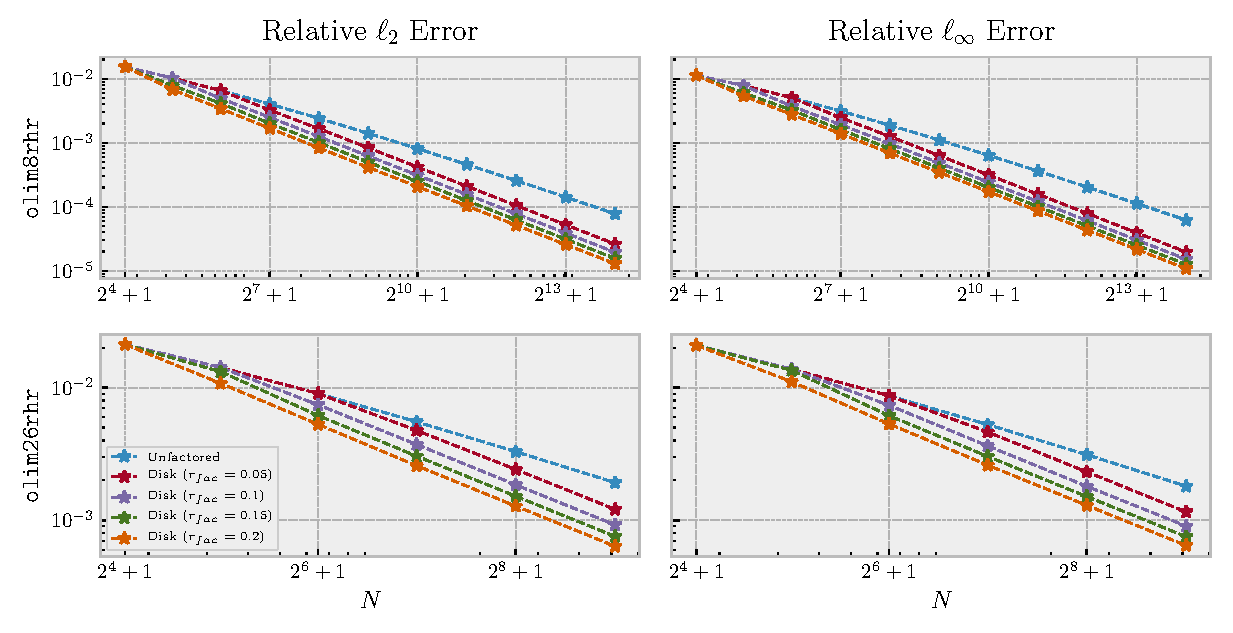
\includegraphics[width=\linewidth]{factoring-error-example.eps}%
  \caption{\emph{Comparing different ways of selecting factored
      nodes.} For the test problem, $\Omega = [-1, 1]^n$, with $n = 2$
    (left) and $n = 3$ (right). The domain is descretized into $N^3$
    nodes, where $N = 2^p + 1$, so that $h = 2/(N - 1)$. The slowness
    function is constant ($s \equiv 1$). For the 2D problem,
    \texttt{olim8rhr} is used; \texttt{olim26rhr} is used for the 3D
    problem. Solutions for the unfactored problem are plotted, along
    with solutions using a disk/sphere neighborhood with constant
    factoring radius given by $\rfac = 0.05, 0.1, 0.15, 0.2$. We note
    that for this problem the choice $\rfac = \sqrt{n}$ results in an
    exact solution. This only applies to the constant slowness
    function, $s \equiv 1$.  }\label{fig:factoring-error-example}
\end{figure}

We consider a problem that has a known analytical solution and has
been used as a test problem for other factored eikonal equation
solvers before\footnote{We thank D.\ Qi for helpful discussions
  regarding this
  problem.}~\cite{slotnick1959lessons,fomel2009fast,qi2018corner}. For
a single point source at $x_i$ and a vector $v$, we define:
\begin{equation}
  \label{eq:slotnick-single-source}
  \frac{1}{s(x)} = \frac{1}{s(x_i)} + v^\top {(x - x_i)},,
\end{equation}
where $s_i = s(x_i)$. The analytic solution to eq.\@
\ref{eq:eikonal} for a single source and slowness function given by
eq.\@ \ref{eq:slotnick-single-source}
is~\cite{slotnick1959lessons}:
\begin{equation}
  \label{eq:slotnick-single-source-solution}
  u_i(x) = \frac{1}{\norm{v}} \cosh^{-1} \parens{1 + \frac{s_i}{2} s(x) \norm{v}^2 \norm{x - x_i}^2}.
\end{equation}
If we shift the point source from $x_i$ to another location $x_j$, we
find:
\begin{equation}
  \label{eq:slotnick-slowness-shift}
  \frac{1}{s_i} + v^\top {(x - x_j + x_j - x_i)} = \frac{1}{s_i} + v^\top {(x_j - x_i)} + v^\top {(x - x_j)} = \frac{1}{s_j} + v^\top {(x - x_j)}.
\end{equation}
That is, the slowness function $s$ remains unchanged as it is
rewritten with respect to a different source.

\begin{figure}
  \centering
  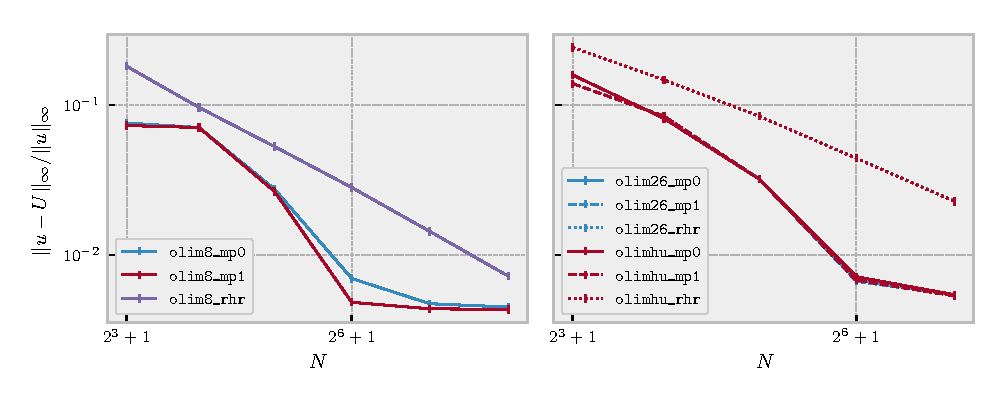
\includegraphics[width=\linewidth]{qv_plots.eps}%
  \caption{Relative $\ell_\infty$ error plotted versus $N$ in 2D
    (left) and 3D (right).}\label{fig:qv}
  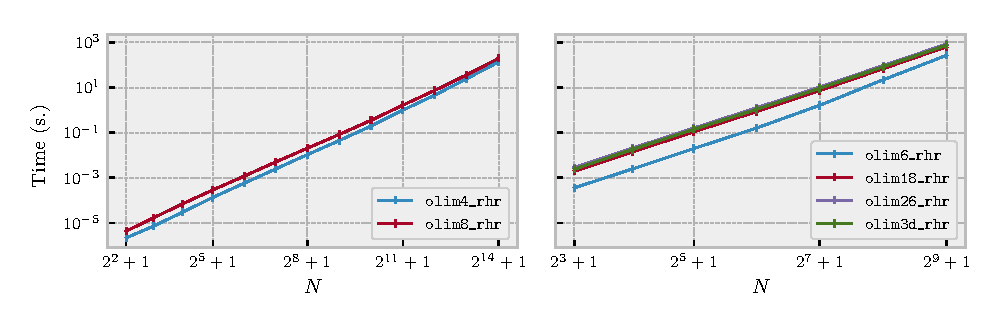
\includegraphics[width=\linewidth]{qv-time-plots.eps}%
  \caption{Wall clock time plotted versus $N$ in 2D (left) and 3D
    (right).}\label{fig:qv-time-plots}
  \caption*{\emph{Numerical results for section\@
      \ref{ssec:slotnick}.} Problem sizes are $N = 2^p + 1$, where
    $p = 3, \hdots, 14$ in 2D and $p = 3, \hdots, 9$ in 3D. The total
    number of nodes is $N^n$, where $n = 2, 3$. See section\@
    \ref{ssec:slotnick} for least squares fits.}
\end{figure}

If $\set{x_i}$ is a set of point sources and $u_i$ is the solution of
the eikonal equation for the single point source problem with point
source given by $x_i$, then the solution for the multiple point source
problem with sources $\set{x_i}$ is:
\begin{equation}
  u(x) = \min_i u_i(x).
\end{equation}
We use this formula to compare relative $\ell_\infty$ errors for each
of our OLIMs in 2D and \texttt{olim26} and \texttt{olim3d} in 3D for
this slowness function with a pair of point sources, $x_1 = (0, 0)$
and $x_2 = (0.8, 0)$ in 2D, and $x_1 = (0, 0, 0)$ and
$x_2 = (0.8, 0, 0)$ in 3D. We set the domain of the problem to be
$\Omega = [0, 1]^n$ and discretize it into $N = 2^p + 1$ points, so
that $h = (N-1)^{-1}$.

For this choice of slowness function, we plot the CPU runtime versus
$N$ (see figure \ref{fig:qv-time-plots}), along with the relative
$\ell_\infty$ error versus $N$ (see figure \ref{fig:qv}). We also do
least squares fits for these plots to get an overall sense of the
accuracy and speed (see \ref{table:qv-least-squares}). Since we have
established that \texttt{olim8}, \texttt{olim26}, and \texttt{olim3d}
are the best choice of neighborhoods in the previous section, we do
not plot these results for \texttt{olim4}, \texttt{olim6}, and
\texttt{olim18}.

We can see that our conclusions from section\@
\ref{ssec:point-source-problems} also hold for the multiple point
source problem. Additionally, our least-squares fits indicate to us
that our algorithms' runtimes are accurately described by the fit
$T_N \sim C_T N^{\alpha}$ with $\alpha \approx n$, and the error by
$E_N \sim C_E h^{\beta}$, with $\beta \approx 1$ (here, $E_N$ is the
relative $\ell_\infty$ error). In fact, for \texttt{olim26} and
\texttt{olim3d} with \texttt{mp0} or \texttt{mp1}, the power $\beta$
is improved beyond $1$ to $\beta \approx 1.3$.

\begin{table}
  \begin{subtable}{0.5\textwidth}
    \centering
    {
      \small
      \begin{tabular}{ccc}
        Neighborhood & $C_T$ & $\alpha$ \\
        \hline \noalign{\vskip 0.2em}
        \texttt{olim4} & $7.779\times 10^{-8}$ & 1.0785 \\
        \texttt{olim8} & $1.971\times 10^{-7}$ & 1.0515 \\
        \hline \noalign{\vskip 0.2em}
        \texttt{olim6} & $2.968\times 10^{-7}$ & 1.085 \\
        \texttt{olim18} & $2.984\times 10^{-6}$ & 1.018 \\
        \texttt{olim26} & $4.649\times 10^{-6}$ & 1.0103 \\
        \texttt{olim3d} & $3.923\times 10^{-6}$ & 1.013 \\
      \end{tabular}
    }
    \caption{$T_N \sim C_T N^{\alpha n}$}
  \end{subtable}%
  \begin{subtable}{0.4999\textwidth}
    \centering
    {
      \small
      \begin{tabular}{ccc}
        Neighborhood & $C_E$ & $\beta$ \\
        \hline \noalign{\vskip 0.2em}
        \texttt{olim8\_mp0} & 0.4077 & 0.98744 \\
        \texttt{olim8\_mp1} & 0.3683 & 0.993 \\
        \texttt{olim8\_rhr} & 1.511 & 0.9728 \\
        \hline \noalign{\vskip 0.2em}
        \texttt{olim26\_mp0} & 2.328 & 1.3135 \\
        \texttt{olim26\_mp1} & 1.949 & 1.2888 \\
        \texttt{olim26\_rhr} & 1.772 & 0.90394 \\
        \hline \noalign{\vskip 0.2em}
        \texttt{olim3d\_mp0} & 2.268 & 1.3141 \\
        \texttt{olim3d\_mp1} & 1.865 & 1.2885 \\
        \texttt{olim3d\_rhr} & 1.77 & 0.90353
      \end{tabular}
    }
    \caption{$E_N \sim C_E h^\beta$}
  \end{subtable}
  \caption{\emph{Least-squares fits of the runtime and relative
      $\ell_\infty$ error for OLIMs in 2D and 3D.} We denote the time
    for a given $N$ by $T_N$; likewise, $E_N$ denotes the relative
    $\ell_\infty$ error for a specific $N$. We fit $T_N$ to a power
    $C_T N^\alpha$. In 2D, we expect $\alpha \approx 2$; in 3D,
    $\alpha \approx 3$. In 3D, we fit $E_N$ to $C_E h^\beta$, and
    expect $\beta \approx -1$ in all cases, due to the use of local
    factoring. In fact, for \texttt{olim26} and \texttt{olim3d} using
    either \texttt{mp0} or \texttt{mp1}, we find that the situation is
    better than expected, with
    $\beta \approx -1.3$.}\label{table:qv-least-squares}
\end{table}

\section{Conclusion}

We have presented two families of fast and accurate direct solvers for
the eikonal equation. One of these relies on enumerating valid update
simplexes, while the other employs a fast search for the first arrival
characteristic. These methods use different quadrature rules: a
simplified midpoint rule (\texttt{mp0}), a midpoint rule
(\texttt{mp1}), and a righthand rule (\texttt{rhr}). We analyze the
relationship between these quadrature rules and prove error bounds. We
conduct numerical experiments measuring runtime and relative
$\ell_\infty$ error. We make a comparison with the standard fast
marching method which is equivalent to our \texttt{olim6\_rhr},
showing that they are comparable in terms of speed and accuracy, with
\texttt{olim6\_rhr} being slightly slower. To determine the relative
time spent on different tasks, we profile our C++ implementation using
Valgrind, separating time spent into several coarse-grained
categories. From this, we show that for practical problem sizes, the
runtime of Dijkstra-like algorithms behaves like $C N^n$, where
$n = 2, 3$, and $N^n$ is the total number of gridpoints (even if this
is not strictly true from a computational complexity viewpoint); we
also emphasize that memory access patterns play a large role in
algorithm runtime, especially for large $N$.

Overall, we conclude that ordered line integral methods are a powerful
approach to obtaining a higher degree of accuracy when solving the
eikonal equation in 3D. With an appropriate choice of quadrature rule,
we are able to exploit improved directional coverage to drive down the
error constant. The improved accuracy more than makes up for the
modest price paid in speed, and we fully expect it to be possible to
find ways to optimize this family of algorithms further. We have also
tried to demonstrate that memory access patterns dominate both update
time and time spent maintaining the front data structure, from which
we can conclude two things: 1) the exact time spent updating a node is
important but not paramount (improving accuracy is more important than
improving speed), 2) using memory optimally will lead to a substantial
speed-up for large problems.

\section{Acknowledgements}

We thank Prof.\ A.\ Vladimirsky for valuable discussions during the
course of this project.

\appendix

\section[Minimum action integral]{Minimum actional integral for the
  eikonal equation}\label{sec:minimum-action-integral} The eikonal
equation eq.\@ \ref{eq:eikonal} is a Hamilton-Jacobi equation for
$u$. If we let each fixed characteristic (ray) of the eikonal equation
be parametrized by some parameter $\sigma$ and denote
$p \equiv \nabla u$, the corresponding Hamiltonian is:
\begin{equation}
  \label{eq:eikonal-hamiltonian}
  H{(p, x)} = \frac{\norm{p}^2}{2} - \frac{s(x)^2}{2} = 0.
\end{equation}
Since $H = 0$, eq.\@ \ref{eq:eikonal-hamiltonian} implies
$L = \sup_p (\langle p, x' \rangle - H) = s(x) \norm{x'}$. Since
$x' = \partial_p H = p$ and $\norm{p} = s(x)$ can be expressed as:
\begin{equation}
  \label{eq:eikonal-lagrangian}
  L(x, x') = \langle p, x'\rangle = \langle x', x'\rangle = \langle \nabla u, x' \rangle = \frac{du}{d\sigma}.
\end{equation}

Let $x(\sigma)$ be a characteristic arriving at
$\hat{x} = x(\hat\sigma)$ from $x_0 = x(0)$, which lies on the
expanding front. Integrating from $0$ to $\hat\sigma$ and letting
$\hat u = u(\hat x)$ and $u_0 = u(x_0)$:
\begin{equation}
  \label{eq:minimum-action-on-a-ray}
  \hat u - u_0 = \int_{0}^{\hat\sigma} L(x, x') d\sigma = \int_{0}^{\hat\sigma} s(x) \norm{x'} d\sigma = \int_0^L s(x) dl,
\end{equation}
where $L$ is the length of the characteristic from $x_0$ to $\hat{x}$
and $dl$ is the length element. A characteristic of eq.\@
\ref{eq:eikonal} minimizes eq.\@ \ref{eq:minimum-action-on-a-ray}
over admissible paths. Then, if $\hat{x}$ is fixed and $\alpha$ is an
arc-length parametrized curve with $\alpha(L) = \hat{x}$, eq.\@
\ref{eq:minimum-action-on-a-ray} is equivalent to:
\begin{equation}\label{eq:eikonal-minimum-action-path}
  \hat{u} = u(\hat{x}) = \min_\alpha \curlyb{u(\alpha(0)) + \int_\alpha s(x) dl}.
\end{equation}
Our update procedure is based on eq.\@
\ref{eq:eikonal-minimum-action-path}. This problem may have multiple
local minima---$\hat{u}$ above corresponds to the first arrival, which
is what interests us primarily in this work. While the standard finite
difference method effectively discretizes the Hamiltonian, the family
of methods presented here discretizes eq.\@
\ref{eq:eikonal-minimum-action-path}.

\section{Proofs for section\@
  \ref{ssec:minimization-problem}}\label{sec:minimization-proofs}

\begin{proof}[Proof of proposition \ref{prop:F0-grad-and-Hess}]
  For the gradient, we have:
  \begin{equation*}
    \nabla F_0(\lambda; \theta) = \delU + \frac{s^{\theta} h}{2 l_\lambda} \nabla p_\lambda^\top p_\lambda = \delU + \frac{s^{\theta} h}{l_\lambda} \delP^\top p_\lambda,
  \end{equation*}
  since
  $\nabla p_\lambda^\top p_\lambda = 2 \delP^\top
  p_\lambda$. For the Hessian:
  \begin{align*}
    \nabla^2_\lambda F_0(\lambda; \theta) &= \nabla \parens{\frac{s^{\theta} h}{l_\lambda} p_\lambda^\top \delP} = s^{\theta} h \parens{\nabla \frac{1}{l_\lambda} p_\lambda^\top \delP + \frac{1}{l_\lambda} \nabla p_\lambda^\top \delP} \\
    &= \frac{s^{\theta} h}{l_\lambda} \parens{\delP^\top \delP - \frac{\delP^\top p_\lambda p_\lambda^\top \delP}{p_\lambda^\top p_\lambda}} = \frac{s^{\theta} h}{l_\lambda} \delP^\top \parens{I - \frac{p_\lambda p_\lambda^\top}{p_\lambda^\top p_\lambda}} \delP,
  \end{align*}
  from which the result follows.
\end{proof}

\begin{proof}[Proof of proposition \ref{prop:F1-grad-and-Hess}]
  Since
  $F_1(\lambda; \theta) = u_\lambda + h s^{\theta}_\lambda l_\lambda$,
  for the gradient we have:
  \begin{equation*}
    \nabla F_1(\lambda; \theta) = \delU + h \parens{\theta l_\lambda \dels + \frac{s^{\theta}_\lambda}{2l_\lambda} \nabla p_\lambda^\top p_\lambda} = \delU + \frac{h}{l_\lambda} \parens{\theta p_\lambda^\top p_\lambda \dels + s^{\theta} \delP^\top p_\lambda},
  \end{equation*}
  and for the Hessian:
  \begin{equation*}
    \begin{aligned}
      \nabla^2 F_1(\lambda; \theta) = \frac{h}{2 l_\lambda} \Bigg(\theta \Big(\nabla p_\lambda^\top p_\lambda \dels^\top &+\; \dels {(\nabla p_\lambda^\top p_\lambda)}^\top\Big) \;+ \\
      &s^{\theta}_\lambda \parens{\frac{1}{2 p_\lambda^\top p_\lambda} \nabla p_\lambda^\top p_\lambda {(\nabla p_\lambda^\top p_\lambda)}^\top - \nabla^2_\lambda p_\lambda^\top p_\lambda} \Bigg).
    \end{aligned}
  \end{equation*}
  Simplifying this gives us the result.
\end{proof}

\begin{proof}[Proof of lemma \ref{lemma:dPt-cprojp-dP-pd}]
  % To show that $\delP^\top \proj^\perp_{p_\lambda} \delP$
  % is positive semidefinite, we simply note that since
  % $\proj^\perp_{p_\lambda}$ is an orthogonal projector, it is
  % positive semidefinite, and its singular value decomposition can be
  % written $UU^\top$, where $U \in \mathbb{R}^{n+1 \times n}$. Then:
  % \begin{equation}\label{eq:dPt-cprojp-dP-gram}
  %   \delP^\top \proj^\perp_{p_\lambda} \delP = {(U^\top \delP)}^\top {(U^\top \delP)}.
  % \end{equation}
  % From the factorization in eq.\@ \ref{eq:dPt-cprojp-dP-gram}, we
  % can see
  % that $\delP^\top \proj^\perp_{p_\lambda} \delP$ is a
  % Gram matrix, hence positive semidefinite.

  Let $\nu_\lambda = p_\lambda/l_\lambda \in \mathbb{R}^n$ be the unit
  vector in the direction of $p_\lambda$, and assume that
  $Q = \begin{bmatrix} \nu_\lambda & U \end{bmatrix} \in \mathbb{R}^{n
    \times n}$ is orthonormal. Then:
  \begin{equation}
    \delP^\top \proj^\perp_{p_\lambda} \delP = \delP^\top {(I - \nu_\lambda \nu_\lambda^\top)} \delP = \delP^\top {(QQ^\top - \nu_\lambda \nu_\lambda^\top)} \delP = \delP^\top U U^\top \delP.
  \end{equation}
  Hence, $\delP^\top \proj^\perp \delP$ is a Gram matrix
  and positive semidefinite.

  Next, since $\Delta^n$ is nondegenerate, the vectors $p_i$ for
  $i = 0, \hdots, n - 1$ are linearly independent. Since the $i$th
  column of $\delP$ is $\delp_i = p_i - p_0$, we can see that
  the vector $p_0$ is not in the range of $\delP$; hence, there is
  no vector $\mu$ such that $\delP \mu = \alpha p_\lambda$, for any
  $\alpha \neq 0$. What's more, by definition,
  $\text{ker}(\proj_{p_\lambda}^\perp) = \langle p_\lambda
  \rangle$. So, we can see that
  $\proj^\perp_{p_\lambda} \delP \mu = 0$ only if $\mu = 0$,
  from which we can conclude
  $\delP^\top \proj^\perp_{p_\lambda} \delP \succ
  0$. Altogether, bearing in mind that $\smin$ is assumed to be
  positive, we conclude that $\nabla^2 F_0$ is positive definite.
\end{proof}

\begin{proof}[Proof of lemma \ref{lemma:F-strictly-convex}]
  To show that $\nabla^2 F_1$ is positive definite for $h$ small
  enough, note from eq.\@ \ref{eq:hess-F1} that $\nabla^2 F_1$ is
  the sum of a positive definite matrix and a small, indefinite
  perturbation. To use this fact, note that since
  $\delP^\top \proj^\perp_\lambda \delP$ is symmetric positive
  definite, it has an eigenvalue decomposition $Q \Lambda Q^\top$
  where $\Lambda_{ii} > 0$ for all $i$. Since
  $\delP^\top \proj^\perp_\lambda \delP$ doesn't depend on $h$,
  for a fixed set of vectors $p_0, \hdots, p_n$, we can expect its
  eigenvalues to be constant with respect to $h$. So, if we write:
  \begin{equation}
    A = \frac{s^\theta_\lambda h}{l_\lambda} \delP^\top \proj^\perp_\lambda \delP = Q \parens{\frac{s^\theta_\lambda h}{l_\lambda} \Lambda} Q^\top
  \end{equation}
  we can expect this matrix's eigenvalues to be $\Theta(h)$; in
  particular, $\lambda_{\min} \geq C h$ for some constant $C$,
  provided that $s > \smin > 0$, as assumed. This gives us a bound for
  the positive definite part of $\nabla F_1^2$.

  The perturbation $B = \set{\delP^\top \nu_\lambda, \theta h \dels}$
  is indefinite. Since $\norm{\dels} = O(h)$, we find that:
  \begin{equation}
    |\lambda_{\max}(B)| = \norm{\anticom{\delP^\top \nu_\lambda,
        \theta h \dels}}_2 \leq \theta h \sqrt{n} \norm{\anticom{\delP^\top \nu_\lambda, \dels}}_\infty = O(h^2),
  \end{equation}
  where we use the fact that the Lipschitz constant of $s$ is
  $K \leq C$, so that:
  \begin{equation}
    |\dels_i| = |s_i - s_0| \leq K |x_i - x_0| \leq K h \sqrt{n}
    \leq Ch \sqrt{n},
  \end{equation}
  for each $i$. Letting $z \neq 0$, we compute:
  \begin{equation}
    z^\top \nabla^2 F_1 z = z^\top A z + z^\top B z \geq \lambda_{\min}(A) z^\top z + z^\top B z \geq Ch z^\top z + z^\top B z.
  \end{equation}
  Now, since
  $\abs{z^\top B z} \leq \abs{\lambda_{\max}(B)} z^\top z \leq D h^2
  z^\top z$, where $D$ is some positive constant, we can see that for
  $h$ small enough, it must be the case that
  $Ch z^\top z + z^\top B z > 0$; i.e., that $\nabla^2 F_1$ is
  positive definite; consequently, $F_1$ is strictly convex in this case.
\end{proof}

\section{Proofs for
  section\@ \ref{ssec:validation}}\label{app:validation-proofs} In this section, we establish some technical lemmas that we will use
to validate the use of \texttt{mp0}. Lemmas
\ref{lemma:bounded-inv-hess-F1}, \ref{lemma:bounded-first-step}, and
\ref{lemma:hess-F1-lipschitz} set up the conditions for theorem
\ref{thm:stoer-bulirsch} of Stoer and
Bulirsch~\cite{stoer2013introduction}, from which theorem
\ref{thm:mp0-newton} readily follows.

\begin{lemma}\label{lemma:bounded-inv-hess-F1}
  There exists $\beta = O(h^{-1})$ s.t.
  $\norm{\nabla^2 F_1(\lambda)^{-1}} \leq \beta$ for all
  $\lambda \in \Delta^n$.
\end{lemma}

\begin{proof}[Proof of lemma \ref{lemma:bounded-inv-hess-F1}]
  To simplify eq.\@ \ref{eq:hess-F1}, we temporarily define:
  \begin{equation}
    A = \frac{s^\theta_\lambda h}{l_\lambda} \delP^\top \proj^\perp_\lambda \delP \mbox{ and } B = \frac{\theta h}{l_\lambda} \anticom{\delP^\top p_\lambda, \dels}.
  \end{equation}
  Observe that $\|A\| = O(h)$ and $\|B\| = O(h^2)$, since
  $\|\delta s\| = O(h)$ and since all other factors involved in $A$
  and $B$ (excluding $h$ itself) are independent of $h$. Hence:
  \begin{equation}
    \norm{A^{-1} B} = \frac{\theta}{s^\theta_\lambda} \norm{\parens{\delP^\top \proj^\perp_\lambda \delP}^{-1} \anticom{\delP^\top p_\lambda, \dels}} = O(h),
  \end{equation}
  since $1/s \leq 1/\smin$ and $\norm{\dels} = O(h)$. Hence,
  $\norm{A^{-1} B} < 1$ for $h$ small enough, and we can Taylor
  expand:
  \begin{equation}
    \begin{aligned}
      \nabla^2 F_1(\lambda)^{-1} &= \parens{A + B}^{-1} = {(I + A^{-1} B)}^{-1} A^{-1} \\
      &= \parens{I - A^{-1} B + {(A^{-1} B)}^2 - \cdots} A^{-1} \\
      &= A^{-1} - A^{-1} B A^{-1} + {(A^{-1} B)}^2 A^{-1} - \,\cdots,
    \end{aligned}
  \end{equation}
  which implies $\norm{\nabla^2 F_1(\lambda)^{-1}} = O(h^{-1})$. Note
  that when we Taylor expand, $\|A^{-1} B\| = O(h)$, so that
  $\|A^{-1} B\| < 1$ for $h$ small enough. To define $\beta$, let:
  \begin{equation}
    \beta = \max_{\lambda \in \Delta^n} \norm{\nabla^2 F_1(\lambda)^{-1}} = O(h^{-1}),
  \end{equation}
  completing the proof.
\end{proof}

\begin{lemma}\label{lemma:bounded-first-step}
  There exists $\alpha = O(h)$ s.t.
  $\norm{\nabla^2 F_1(\lambda_{0}^*)^{-1} \nabla F_1(\lambda_{0}^*)}
  \leq \alpha$.
\end{lemma}

\begin{proof}[Proof of lemma \ref{lemma:bounded-first-step}]
  From lemma \ref{lemma:bounded-inv-hess-F1} we have
  $\norm{F_1(\lambda_0^*)^{-1}} = O(h^{-1})$, so to establish the
  result we only need to show that
  $\norm{\nabla F_1(\lambda_0^*)} = O(h^2)$. To this end, let
  $\underline{\lambda} = {(n + 1)}^{-1} \m{1}_{n \times 1}$ (i.e., the
  centroid of $\Delta^n$, where $s^\theta$ is evaluated). Then,
  recalling figure \ref{fig:simplex-diagrams},
  $s^\theta_\lambda = s^\theta + \dels^\top (\lambda -
  \underline{\lambda})$ so that, for a general $\lambda$:
  \begin{equation}\label{eq:grad-F1-in-terms-of-grad-F0}
    \begin{aligned}
      \nabla F_1(\lambda) &= l_\lambda h \dels + \delU + \frac{s^\theta + \dels^\top (\lambda - \underline{\lambda})}{l_\lambda} h \delP^\top p_\lambda \\
      &= l_\lambda h \dels + \nabla F_0(\lambda) + \frac{\dels^\top {(\lambda - \underline{\lambda})}}{l_\lambda} h \delP^\top p_\lambda.
    \end{aligned}
  \end{equation}
  Since $\nabla F_0(\lambda_0^*) = 0$ by optimality, we can conclude
  using eq.\@ \ref{eq:grad-F1-in-terms-of-grad-F0} and
  $\norm{\dels} = O(h)$ that:
  \begin{equation}
    \norm{\nabla F_1(\lambda_0^*)} = h \norm{l_{\lambda_0^*} \dels + \frac{\dels^\top {(\lambda - \underline{\lambda})}}{l_{\lambda_0^*}} \delP^\top p_\lambda} = O(h^2),
  \end{equation}
  which proves the result.
\end{proof}

\begin{lemma}\label{lemma:hess-F1-lipschitz}
  The Hessian $\nabla^2 F_1$ is Lipschitz continuous with $O(h)$
  Lipschitz constant. That is, there is some constant $\gamma = O(h)$
  so that for two points $\lambda$ and $\lambda'$:
  \begin{align*}
    \norm{\nabla^2 F_1(\lambda) - \nabla^2 F_1(\lambda')} \leq \gamma \norm{\lambda - \lambda'}.
  \end{align*}
\end{lemma}

\begin{proof}[Proof of lemma \ref{lemma:hess-F1-lipschitz}]
  If we restrict our attention to $\Delta^n$, we see that
  $l_\lambda^{-1} \delP^\top \proj_\lambda^\perp \delP$ is
  Lipschitz continuous function of $\lambda$ with $O(1)$ Lipschitz
  constant and $\theta \{{\delP}^\top p_\lambda, \dels\} /l_{\lambda}$
  is Lipschitz continuous with $O(h)$ Lipschitz constant since
  $\|\delta s\| = O(h)$. Then, since $s^\theta_\lambda$ is $O(1)$
  Lipschitz, it follows that:
  \begin{equation}
    A(\lambda) = \tfrac{s^\theta_\lambda h}{l_\lambda} \delP^\top
    \proj^\perp_\lambda \delP
  \end{equation}
  has a Lipschitz constant that is $O(h)$ for $\lambda \in \Delta^n$,
  using the notation of lemma
  \ref{lemma:bounded-inv-hess-F1}. Likewise,
  \begin{equation}
    B(\lambda) = \tfrac{\theta h}{l_\lambda} \anticom{\delP^\top
      p_\lambda, \dels} = O(h^2),
  \end{equation}
  since it is a sum of two terms involving products of $h$ and
  $\delta s$. Since $\nabla^2 F_1(\lambda) = A(\lambda) + B(\lambda)$,
  we can see immediately that it is also Lipschitz on $\Delta^n$ with
  a constant that is $O(h)$.
\end{proof}

\begin{proof}[Proof of theorem \ref{thm:mp0-newton}]
  Our proof of theorem \ref{thm:mp0-newton} relies on the following
  theorem on the convergence of Newton's method, which we present for
  convenience.

  \begin{theorem}[Theorem 5.3.2, Stoer and Bulirsch]\label{thm:stoer-bulirsch}
    Let $C \subseteq \R^n$ be an open set, let $C_0$ be a convex set
    with $\overline{C}_0 \subseteq C$, and let
    $f : C \to \mathbb{R}^n$ be differentiable for $x \in C_0$ and
    continuous for $x \in C$. For $x_0 \in C_0$, let
    $r, \alpha, \beta, \gamma$ satisfy
    $S_r(x_0) = \set{x : \norm{x - x_0} < r} \subseteq C_0$,
    $\mu = \alpha\beta\gamma < 2$, $r = \alpha(1 - \mu)^{-1}$, and let
    $f$ satisfy:
    \begin{enumerate}[label=(\alph*)]
    \item for all $x, y \in C_0$,
      $\norm{D f(x) - D f(y)} \leq \gamma \norm{x - y}$,
    \item for all $x \in C_0$, $(D f(x))^{-1}$ exists and satisfies
      $\norm{(Df(x))^{-1}} \leq \beta$,
    \item and $\norm{(Df(x_0))^{-1} f(x_0)} \leq \alpha$.
    \end{enumerate}
    Then, beginning at $x_0$, each iterate:
    \begin{equation}
      x_{k+1} = x_k - Df(x_k)^{-1} f(x_k), \qquad k = 0, 1, \hdots,
    \end{equation}
    is well-defined and satisfies $\norm{x_k - x_0} < r$ for all
    $k \geq 0$. Furthermore, $\lim_{k \to \infty} x_k = \xi$ exists and
    satisfies $\norm{\xi - x_0} \leq r$ and $f(\xi) = 0$.
  \end{theorem}

  For our situation, Theorem 5.3.2 of Stoer and
  Bulirsch~\cite{stoer2013introduction} indicates that if:
  \begin{align}
    \|\nabla F_1(\lambda)^{-1}\| &\leq \beta, \mbox{where } \beta = O(h^{-1}) \label{enum:sb-newton-1}, \\
    \|\nabla F_1(\lambda_0^*)^{-1} \nabla F_1(\lambda_0^*)\| &\leq \alpha, \mbox{where } \alpha = O(h), \label{enum:sb-newton-2} \mbox{ and} \\
    \|\nabla F_1(\lambda) - \nabla F_1(\lambda')\| &\leq \gamma \norm{\lambda - \lambda'} \mbox{ for each } \lambda, \lambda' \in \Delta^n, \mbox{where } \gamma = O(h), \label{enum:sb-newton-3}
  \end{align}
  then with $\lambda_0 = \lambda_0^*$, the iteration eq.\@
  \ref{eq:lam0-iter-to-lam1} is well-defined, with each iterate
  satisfying $\norm{\lambda_k - \lambda_0} \leq r$, where
  $r = \alpha/(1 - \alpha\beta\gamma/2)$. Additionally, the limit of
  this iteration exists, and the iteration converges to it
  quadratically; we note that since $F_1$ is strictly convex for $h$
  small enough, the limit of the iteration must be $\lambda_1^*$, so
  the theorem also gives us
  $\norm{\dellam^*} = \norm{\lambda_1^* - \lambda_0^*} \leq r$.

  Now, we note that items \ref{enum:sb-newton-1},
  \ref{enum:sb-newton-2}, and \ref{enum:sb-newton-3} correspond
  exactly to lemma \ref{lemma:bounded-inv-hess-F1},
  \ref{lemma:bounded-first-step}, and \ref{lemma:hess-F1-lipschitz},
  respectively which gave us values for $\alpha, \beta$, and
  $\gamma$. All that remains is to compute $r$. Since the preceding
  lemmas imply $\alpha\beta\gamma = O(h)$, hence
  $\alpha\beta\gamma/2 < 1$ for $h$ small enough. We have:
  \begin{equation}
    r = \frac{\alpha}{1 - \frac{\alpha\beta\gamma}{2}} = \alpha \parens{1 + \frac{\alpha\beta\gamma}{2} + \frac{\alpha^2\beta^2\gamma^2}{4} + \cdots} = O(h),
  \end{equation}
  so that $\norm{\dellam^*} = O(h)$, and the result follows.

  To obtain the $O(h^3)$ error bound, from theorem
  \ref{thm:mp0-newton}, we have $\norm{\dellam^*} = O(h)$. Then,
  Taylor expanding $F_1(\lambda_0^*)$, we get:
  \begin{equation*}
    F_1(\lambda_0^*)
    = F_1(\lambda_1^* - \dellam^*) = F_1(\lambda_1^*) - \nabla F_1(\lambda_1^*)^\top \dellam^* + \frac{1}{2} \dellam^* \nabla F_1^2(\lambda_1^*) \dellam^* + R,
  \end{equation*}
  where $\abs{R} = O(\norm{\dellam^*}^3)$. Since $\lambda_1^*$
  is optimum, $\nabla F_1(\lambda_1^*) = 0$. Hence:
  \begin{equation*}
    \abs{F_1(\lambda_1^*) - F_1(\lambda_0^*)} \leq \frac{1}{2} \norm{\nabla F_1^2(\lambda_1^*)} \norm{\dellam^*}^2 + O(\norm{\dellam^*}^3) = O(h^3),
  \end{equation*}
  which proves the result.
\end{proof}

\section{Proofs for section\@
  \ref{ssec:exact-soln}}\label{sec:exact-soln-proofs}

\begin{figure}
  \vspace{1em}
  \centering 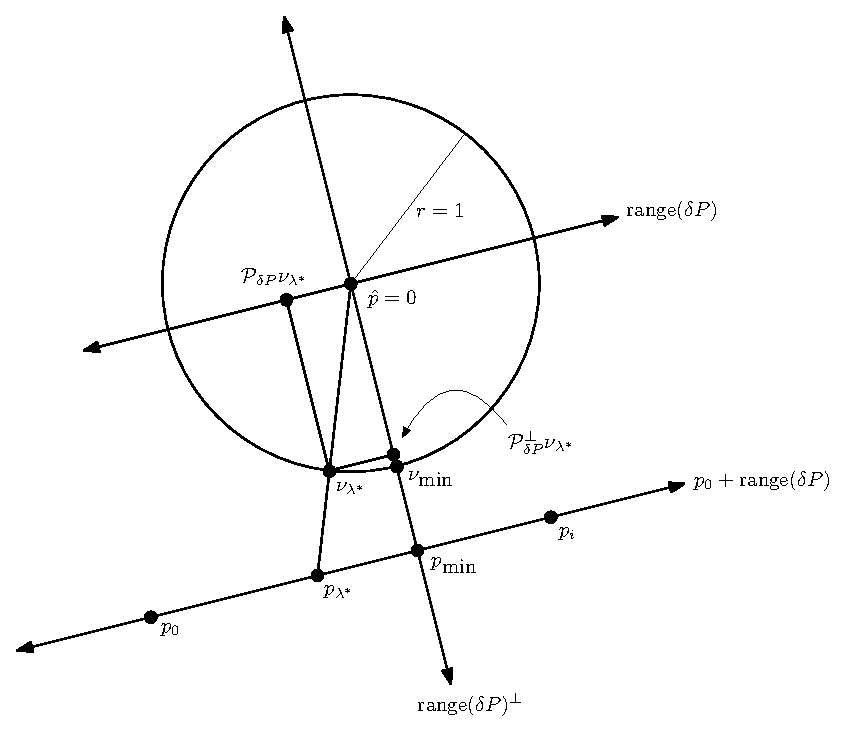
\includegraphics[width=0.8\linewidth]{f0-exact.eps}
  \caption{A schematic depiction of the proof of theorem
    \ref{thm:f0-exact}.}\label{fig:f0-exact}
\end{figure}

\begin{proof}[Proof of theorem \ref{thm:f0-exact}]
  We proceed by reasoning geometrically; figure \ref{fig:f0-exact}
  depicts the geometric setup. First, letting $\delP = QR$ be the
  reduced QR decomposition of $\delP$, and writing
  $\nu_{\lambda^*} = p_{\lambda^*}/l_{\lambda^*}$, we note that since:
  \begin{equation}
    \nabla F_0(\lambda^*) = \delU + s^\theta h \delP^\top \nu_{\lambda^*} = 0,
  \end{equation}
  the optimum $\lambda^*$ satisfies:
  \begin{equation}\label{eq:Qt-n}
    - R^{-\top} \frac{\delU}{s^\theta h} = Q^\top \nu_{\lambda^*}
  \end{equation}
  Let $\proj_{\delP} = QQ^\top$ denote the orthogonal
  projector onto $\range(\delP)$, and
  $\proj^\perp_{\delP} = I - QQ^\top$ the projector onto its
  orthogonal complement. We can try to write $p_{\lambda^*}$ by
  splitting it into a component that lies in $\range(\delP)$ and
  one that lies in $\range(\delP)^\perp$. Letting $\pmin$ be the
  point in $p_0 + \range(\delP)$ with the smallest 2-norm, we
  write:
  \begin{equation}\label{eq:plam-decomp}
    p_{\lambda^*} = (p_{\lambda^*} - \pmin) + \pmin,
  \end{equation}
  where $p_{\lambda^*} - \pmin \in \range(\delP)$ and
  $\pmin \in \range(\delP)^\perp$. The vector $\pmin$ corresponds to
  $p_{\lambdamin}$ where $\lambdamin$ satisfies:
  \begin{equation}
    0 = \delP^\top (\delP \lambdamin + p_0) = R^\top R \lambdamin + R^\top Q^\top p_0,
  \end{equation}
  hence $\lambdamin = -R^{-1} Q^\top p_0$, giving us:
  \begin{equation}\label{eq:pmin}
    \pmin = p_0 + \delP \lambdamin = \proj^\perp_{\delP} p_0.
  \end{equation}
  This vector is easily obtained. For $p_{\lambda^*} - \pmin$, we note
  that $\proj_{\delP} \nu_{\lambda^*}$ is proportional to
  $p_{\lambda^*} - \pmin$, suggesting that we determine the ratio
  $\alpha$ satisfying
  $p_{\lambda^*} - \pmin = \alpha \proj_{\delP}
  \nu_{\lambda^*}$. In particular, from the similarity of the
  triangles
  $(\hat{p}, \nu_{\lambda^*}, \proj^\perp_{\delP}
  \nu_{\lambda^*})$ and $(\hat{p}, p_{\lambda^*}, \pmin)$ in figure
  \ref{fig:f0-exact}, we have, using eqs.\@ \ref{eq:Qt-n} and
  \ref{eq:pmin}:
  \begin{equation}\label{eq:alpha-solve}
    \alpha = \frac{\norm{\pmin}}{\norm{\proj^\perp_{\delP} \nu_{\lambda^*}}} = \sqrt{\frac{p_0^\top \proj^\perp_{\delP} p_0}{1 - \norm{Q^\top \nu_{\lambda^*}}^2}} = \sqrt{\frac{p_0^\top \proj^\perp_{\delP} p_0}{1 - \norm{R^{-\top} \frac{\delU}{s^\theta h}}^2}}.
  \end{equation}
  At the same time, since:
  \begin{equation}
    \nu_{\lambda^*}^\top \proj^\perp_{\delP} \nu_{\lambda^*} = \frac{{(\proj^\perp_{\delP} p_{\lambda^*})}^\top {(\proj^\perp_{\delP} p_{\lambda^*})}}{l_{\lambda_*}^2} = \frac{\pmin^\top \pmin}{l_{\lambda^*}^2} = \frac{p_0^\top \proj^\perp_{\delP} p_0}{l_{\lambda^*}^2}
  \end{equation}
  we can conclude that:
  \begin{equation}
    l_{\lambda^*} = \alpha = \sqrt{\frac{p_0^\top \proj^\perp_{\delP} p_0}{1 - \norm{R^{-\top} \frac{\delU}{s^\theta h}}^2}},
  \end{equation}
  giving us eq.\@ \ref{eq:l-star-expression}, proving the first
  part of theorem \ref{thm:f0-exact}.

  Next, combining eqs.\@ \ref{eq:Qt-n}, \ref{eq:plam-decomp},
  \ref{eq:pmin}, and \ref{eq:alpha-solve}, we get:
  \begin{equation}\label{eq:plam-final}
    p_{\lambda^*} = \proj^\perp_{\delP} p_0 - \sqrt{\frac{p_0^\top \proj^\perp_{\delP} p_0}{1 - \norm{R^{-\top} \frac{\delU}{s^\theta h}}^2}} Q R^{-\top} \frac{\delU}{s^\theta h}.
  \end{equation}
  This expression for $p_{\lambda^*}$ can be computed from our problem
  data and $\delP$. Now, note that
  $p_{\lambda^*} = p_0 + \delP \lambda^*$ implies:
  \begin{equation}\label{eq:lambda-1}
    \lambda^* = R^{-1} Q^\top (p_{\lambda^*} - p_0).
  \end{equation}
  Substituting eq.\@ \ref{eq:plam-final} into eq.\@
  \ref{eq:lambda-1}, we obtain eq.\@ \ref{eq:f0-exact-lambda} after
  making appropriate cancellations, establishing the second part of
  theorem \ref{thm:f0-exact}.

  To establish eq.\@ \ref{eq:f0-exact}, we note that by optimality
  of $\lambda^*$, our expression for $\nabla F_0$ (eq.\@
  \ref{eq:F0-grad} of proposition \ref{prop:F0-grad-and-Hess}) gives:
  \begin{equation}
    \delU = -s^\theta h \frac{\delP^\top p_{\lambda^*}}{l_{\lambda^*}}.
  \end{equation}
  This lets us write:
  \begin{equation}\label{eq:delta-U-dot-lambda-star}
    \delU^\top \lambda^* = -\frac{s^\theta h}{l_{\lambda^*}} p_{\lambda^*}^\top \delP^\top \lambda^* = \frac{s^\theta h}{l_{\lambda^*}} p_{\lambda^*}^\top {(p_0 - p_{\lambda^*})}.
  \end{equation}
  Combining eq.\@ \ref{eq:delta-U-dot-lambda-star} with our
  definition of $F_0$ yields:
  \begin{equation}
    \hat{U} = F_0(\lambda^*) = U_0 + \delU^\top \lambda^* + s^\theta h l_{\lambda^*} = U_0 + \frac{s^\theta h}{l_{\lambda^*}} p_{\lambda^*}^\top {(p_0 - p_{\lambda^*})} + \frac{s^\theta h}{l_{\lambda^*}} p_{\lambda^*}^\top p_{\lambda^*},
  \end{equation}
  which gives eq.\@ \ref{eq:f0-exact}, completing the final part of
  the proof.
\end{proof}

\section{Proofs for section\@ \ref{ssec:equivalence}}\label{sec:equivalence-proofs}

\begin{proof}[Proof of theorem \ref{thm:equivalence}]
  We assume that $U$ is a linear function in the update simplex;
  hence, $\nabla U$ is constant. By stacking and subtracting eq.\@
  \ref{eq:finite-differences} for different values of $i$, we obtain,
  for $i = 0, \hdots, n - 1$:
  \begin{equation}\label{eq:finite-diff-eq}
    \begin{bmatrix}
      \delP^\top \\
      p_i^\top
    \end{bmatrix} \nabla U = \begin{bmatrix}
      \delU \\
      U_0 - \hat{U}
    \end{bmatrix}.
  \end{equation}
  The inverse of the matrix in the left-hand side of eq.\@
  \ref{eq:finite-diff-eq} is:
  \begin{equation}
    \begin{bmatrix}
      \parens{I - \frac{\numin p_i^\top}{\numin^\top p_i}} Q R^{-\top}, &
      \frac{\numin}{\numin^\top p_i}
    \end{bmatrix},
  \end{equation}
  which can be checked. This gives us:
  \begin{equation}
    \nabla U = \parens{I - \frac{\numin p_i^\top}{\numin^\top p_i}} Q R^{-\top} \delU + \frac{U_i - \hat{U}}{\numin^\top p_i} \numin.
  \end{equation}
  Hence, $\|\nabla U\|^2$ is a quadratic equation in
  $\hat{U} - U_i$. Expanding $\|\nabla U\|^2$, a number of
  cancellations occur since $Q^\top \numin = 0$. We have:
  \begin{equation}
    \delU^\top R^{-1} Q^\top \hspace{-0.25em} \parens{I - \frac{\numin p_i^\top}{\numin^\top p_i}}^{\hspace{-0.25em}\top} \hspace{-0.4em} \parens{I - \frac{\numin p_i^\top}{\numin^\top p_i}} \hspace{-0.1em} Q R^{-\top} \delU = \norm{R^{-\top} \delU}^2 + \frac{\parens{p_i^\top Q R^{-\top} \delU}^2}{\norm{\pmin}^2},
  \end{equation}
  so that, written in standard form:
  \begin{equation}
    \begin{aligned}
      {(\hat{U} - U_i)}^2 + 2 p_i^\top Q R^{-\top} \delU {(\hat{U} - U_i)} \,&+\, \parens{p_i^\top Q R^{-\top} \delU}^2 + \\
       &\norm{\pmin}^2 \parens{\norm{R^{-\top} \delU}^2 - \parens{s^\theta h}^2} = 0.
    \end{aligned}
  \end{equation}
  Solving for $\hat{U} - U_i$ gives:
  \begin{equation}
    \hat{U} = U_i - p_i^\top Q R^{-\top} \delU + \norm{\pmin} \sqrt{\parens{s^\theta h} - \|R^{-\top} \delU\|^2},
  \end{equation}
  establishing eq.\@ \ref{eq:U-finite-diff}.

  Next, to show that $\hat{U}' = \hat{U}$, we compute:
  \begin{align*}
    \hat{U}'
    &= U_0 + \delU^\top \lambda^* + s^\theta h l_{\lambda^*} & \mbox{(eq.\@ \ref{eq:f0-definition})} \\
    &= U_0 - \parens{Q^\top p_0 + l_{\lambda^*} R^{-\top} \frac{\delU}{s^\theta h}}^\top R^{-\top} \delU + s^\theta h l_{\lambda^*} & \mbox{(eq.\@ \ref{eq:f0-exact-lambda})} \\
    &= U_0 - p_0^\top Q R^{-\top} \delU + s^\theta h l_{\lambda^*} \parens{1 - \norm{R^{-\top} \frac{\delU}{s^\theta h}}^2} \\
    &= U_0 - p_0^\top Q R^{-\top} \delU + \norm{\pmin} \sqrt{\parens{s^\theta h}^2 - \norm{R^\top \delU}^2} = \hat{U}. & \mbox{(eq.\@ \ref{eq:l-star-expression})}
  \end{align*}
  To establish eq.\@ \ref{eq:U-from-Ui-exact}, first note that
  $-R^{-\top} \delU = s^\theta h Q^\top \nu_{\lambda^*}$ by
  optimality. Substituting this into eq.\@ \ref{eq:U-finite-diff},
  we first obtain:
  \begin{equation}
    \hat{U} = U_i + \frac{s^\theta h}{l_{\lambda^*}} \parens{p_i^\top \proj_{\delP} p_{\lambda^*} + \norm{\pmin} \sqrt{p_{\lambda^*}^\top \proj^\perp_{\delP} p_{\lambda^*}}}.
  \end{equation}
  Now, using the notation for weighted norms and inner products, we have:
  \begin{equation}\label{eq:weighted-norms}
    p_i^\top \proj_{\delP} p_{\lambda^*} + \norm{\pmin} \sqrt{p_{\lambda^*}^\top \proj^\perp_{\delP} p_{\lambda^*}} = \langle p_i, p_{\lambda^*} \rangle_{\proj_{\delP}} + \norm{p_i}_{\proj^\perp_{\delP}} \norm{p_{\lambda^*}}_{\proj^\perp_{\delP}}.
  \end{equation}
  Since $\proj^\perp_{\delP}$ orthogonally projects onto
  $\range(\delP)^\perp$, and since the dimension of this subspace is
  1, $\proj^\perp_{\delP} p_i$ and
  $\proj^\perp_{\delP} p_{\lambda^*}$ are multiples of one
  another and their directions coincide (see figure
  \ref{fig:f0-exact}); furthermore, the angle between them is since
  our simplex is nondegenerate. So, by Cauchy-Schwarz:
  \begin{equation}\label{eq:cauchy-schwarz}
    \norm{p_i}_{\proj^\perp_{\delP}} \norm{p_{\lambda^*}}_{\proj^\perp_{\delP}} = \langle p_i, p_{\lambda^*} \rangle_{\proj^\perp_{\delP}}.
  \end{equation}
  Combining eq.\@ \ref{eq:cauchy-schwarz} with eq.\@
  \ref{eq:weighted-norms} and cancelling terms yields:
  \begin{equation}
    p_i^\top \proj_{\delP} p_{\lambda^*} + \norm{\pmin} \sqrt{p_{\lambda^*}^\top \proj_{\delP} p_{\lambda^*}} = p_i^\top p_{\lambda^*}.
  \end{equation}
  Eq.\@ \ref{eq:U-from-Ui-exact} follows.

  To parametrize the characteristic found by solving the finite
  difference problem, first note that the characteristic arriving at
  $\hat{p}$ is colinear with $\nabla \hat{U}$. If we let $\tilde{\nu}$
  be the normal pointing from $\hat{p}$ in the direction of the
  arriving characteristic, let $\tilde{p}$ be the point of
  intersection between
  $p_0 + \range(\delP)$ and
  $\operatorname{span}\hspace{-0.15em}{(\tilde{\nu})}$, and let
  $\tilde{l} = \norm{\tilde{p}}$, then, since
  $\tilde{p} - p_0 \in \range(\delP)$:
  \begin{equation}
    \numin^\top (\tilde{p} - p_0) = 0.
  \end{equation}
  Rearranging this and substituting
  $\tilde{p} = \tilde{l} \tilde{\nu}$, we get:
  \begin{equation}
    \tilde{l} = \frac{\numin^\top p_0}{\numin^\top \tilde{\nu}}.
  \end{equation}
  Now, if we assume that we can write
  $\tilde{p} = \delP \tilde{\lambda} + p_0$ for some
  $\tilde{\lambda}$, then:
  \begin{equation}
    \tilde{\lambda} = R^{-1} Q^\top \parens{\tilde{p} - p_0} = -R^{-1} Q^\top \parens{I - \frac{\tilde{\nu} \numin^\top}{\tilde{\nu}^\top \numin}} p_0.
  \end{equation}

  To see that $\tilde{p} = p_{\lambda^*}$, note that since
  $\tilde{\nu} = -\nabla \hat{U}/\norm{\nabla \hat{U}} = -\nabla
  \hat{U}/(s^\theta h)$:
  \begin{equation}
    \proj_{\delP} \tilde{\nu} = \frac{-\proj_{\delP} \nabla \hat{U}}{s^\theta h} = \frac{-QR^{-\top} \delU}{s^\theta h} = \proj_{\delP} \nu_{\lambda^*}.
  \end{equation}
  Since $\tilde{\nu}$ and $\nu_{\lambda^*}$ each lie in the unit
  sphere on the same side of the hyperplane spanned by $\delP$, and
  since $\proj_{\delP}$ orthogonally projects onto
  $\range(\delP)$, we can see that in fact
  $\tilde{\nu} = \nu_{\lambda^*}$. Hence,
  $\tilde{p} = p_{\lambda^*} \in p_0 + \range(\delP)$. The second and
  third parts of theorem \ref{thm:equivalence} follow.
\end{proof}

\section{Proofs for section\@
  \ref{ssec:causality}}\label{sec:causality-proofs}

\begin{proof}[Proof of theorem \ref{thm:causality}]
  For causality of $F_0$, we want $\hat{U} \geq \max_i U_i$, which is
  equivalent to $\min_i(\hat{U} - U_i) \geq 0$. From eq.\@
  \ref{eq:U-finite-diff}, we have:
  \begin{equation}
    \min_i \parens{\hat{U} - U_i} = s^\theta h \min_i \min_{\lambda \in \Delta^n} \frac{\nu_i^\top \nu_{\lambda}}{\norm{p_\lambda}} = s^\theta h \min_{i, j} \frac{\nu_i^\top \nu_j}{\norm{p_i}} \geq 0.
  \end{equation}
  The last equality follows because minimizing the cosine between two
  unit vectors is equivalent to maximizing the angle between them;
  since $\lambda$ is restricted to lie in $\Delta^n$, this clearly
  happens at a vertex since the minimization problem is a linear
  program.

  For $F_1$, first rewrite $s_\lambda^\theta$ as follows:
  \begin{equation}
    s_\lambda^\theta = s^\theta + \theta (s_0 + \dels^\top \lambda - \overline{s}),
  \end{equation}
  where $\overline{s} = n^{-1} \sum_{i=0}^{n-1} s_i$. If
  $\lambda_0^\star$ and $\lambda_1^\star$ are the minimizing arguments
  for $F_0$ and $F_1$, respectively, and if
  $\dellam^* = \lambda_1^* - \lambda_0^*$, then we have:
  \begin{equation}\label{eq:F1-in-terms-of-F0}
    F_1^\theta(\lambda_1^*) = F_0^\theta(\lambda_1^*) + \theta \parens{s_0 + \dels^\top \lambda_1^* - \overline{s}} h l_{\lambda_1^\star}.
  \end{equation}
  By the optimality of $\lambda_0^*$ and strict convexity of
  $F_0^\theta$ (lemma \ref{lemma:F-strictly-convex}), we can Taylor
  expand and write:
  \begin{equation}
    F_0^\theta(\lambda_1^*) = F_0^\theta(\lambda_0^*) + \nabla F_0^\theta(\lambda_0^*)^\top \dellam^* + \frac{1}{2} {\dellam^*}^\top \nabla^2 F_0^\theta(\lambda_0^*) \dellam^* + R \geq R,
  \end{equation}
  where $\abs{R} = O(h^3)$ by theorem \ref{thm:mp0-newton}. Let
  $\hat{U} = F_1^\theta(\lambda_1^*)$. Since $F_0^\theta$ is causal,
  we can write:
  \begin{equation}
    \hat{U} \geq \max_i U_i + R + \theta \parens{s_0 + \dels^\top \lambda_1^* - \overline{s}} h l_{\lambda_1^*}.
  \end{equation}
  Since $s$ is Lipschitz, the last term is $O(h^2)$---in particular,
  $\norm{\dels} = O(h)$ and $\norm{s_0 - \overline{s}} = O(h)$ since
  $s_0$ and $\overline{s}$ lie in the same simplex. So, because the
  gap $\min_i(\hat{U} - U_i)$ is $O(h^2)$, we can see that
  $\hat{U} \geq \max_i U_i$ for $h$ sufficiently small.
\end{proof}

\bibliographystyle{plain}
\bibliography{eikonal}{}

\end{document}

%%% Local Variables:
%%% mode: latex
%%% TeX-master: t
%%% End:
